\section{The Large Hadron Collider}
%* Overview of LHC and experiments at the interaction points
The Large Hadron Collider \cite{LHC:LHC} (LHC) is a two-ring proton-proton and Pb-Pb ion collider installed into the 27km long LEP tunnel at CERN. The primary discovery goal of the LHC was the observation of the Higgs boson which was achieved in July 2012 \cite{Atlas:higgs}. The LHC has two high-luminosity experiments, ATLAS \cite{Atlas:design} and CMS \cite{LHC:CMS} with a design peak luminosity of $10^{34}\text{cm}^{-2}\text{s}^{-1}$, in addition to TOTEM \cite{LHC:TOTEM}, LHCb \cite{LHC:LHCb}, and ALICE \cite{LHC:ALICE}. 

%showing the different beam Insertion Regions (IR) corresponding to 
The proton source for the LHC is a bottle of hydrogen gas. The hydrogen is ionised by an electric field before they are accelerated to around 50\MeV by Linac 2. The Proton Synchrotron (PS) PS accelerates protons to 25\GeV and provides them as bunches with a 25ns spacing to the Super Proton Synchrotron (SPS). The SPS accelerates the bunches to an energy of 450\GeV. The acceleration of proton bunches in the LHC itself is achieved through the radio frequency (RF) system. The RF system is comprised of 16 RF cavities housed in 4 cryomodules. Each RF cavity delivers an oscillating longitudinal electric field of 5MV/m, delivering an accelerating voltage of 2MV at a frequency of 400MHz. The RF cavities serve two primary purposes, first to accelerate the protons with every pass of the RF system, and second to group the packets of  protons from the PS into even tighter bunches, to ensure a high luminosity at the collision points. The proton injection is timed such that the center of a packet of protons is located just after the oscillating field maximum. Hence, protons just before the center of the bunch (closer to the field maximum) will be accelerated more than protons just after the center of the bunch (further from the field maximum). This results in protons away from the center of the bunch to be moved towards the center, creating stable, tight, bunches. The number of possible stable bunches ($h$) is therefore equal to the number of possible synchronised protons. A proton is synchronised if the RF frequency ($f_{\text{RF}}$) is an integer multiple of the revolution frequency ($f_{\text{rev}}$)
\begin{equation}
    f_{\text{RF}}=h\times f_{\text{rev}}.
\end{equation}
Therefore dividing the two frequencies gives the number of possible bunches. With $f_{\text{rev}}=c/27$km and $f_{\text{RF}}=400$MHz, this gives the value of $h$ as approximately 35640. These are called RF buckets. Not every RF bucket is filled, and the number of occupied buckets in the LHC is 2808. Each bunch contains $\sim \num{1.15e11}$ protons \cite{LHC:design,LHC:acceleratorspedestrians,LHC:rfcavities}. A schematic of the CERN accelerator complex is shown in Figure \ref{fig:LHC:ccc}.
\begin{figure}[t]
    \centering
    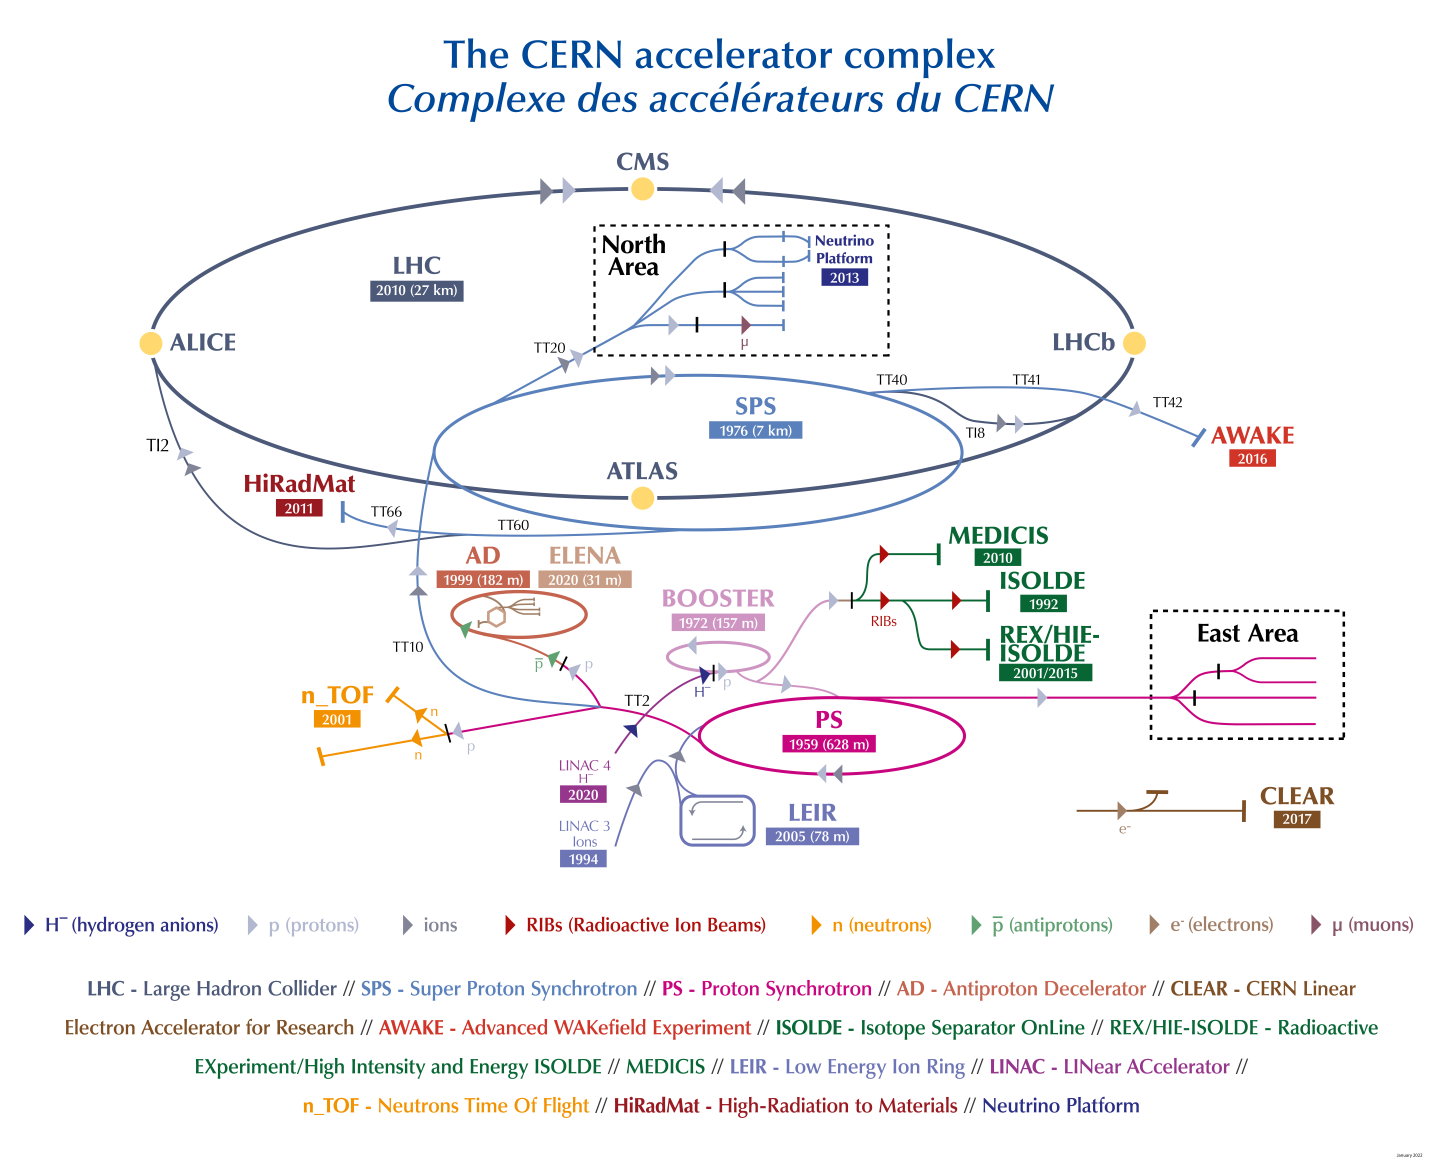
\includegraphics[width=\textwidth]{plots/lhc/CCC-v2022.png}
    \caption{The CERN accelerator complex. Figure taken from \cite{LHC:CCC}.\label{fig:LHC:ccc}}
\end{figure}

As protons carry electric charge, the particle beam will naturally diverge. In the curved sections of the LHC (arcs), the beam must be focused such that its width and height are constrained to be within the vacuum chamber. At the interaction Points (IPs), to enhance the interaction probability for each bunch crossing, the beams are focussed to a size of 16$\mu$m in the $x-y$ plane for CMS and ATLAS. The focussing in the arcs is achieved by collections of superconducting quadrupole, dipole, and other multipole magnets organised into twenty-three LHC cells per arc, resulting in a total of 858 quadrupoles and 1232 dipoles. For the 1232 superconducting dipoles to operate reliably at the 8.33T magnetic field required for 7 TeV beams, the magnet system must operate in a bath of superfluid helium at a temperature of 1.9K. Dispersion suppressors, comprised of four quadrupoles separated by two dipole magnets, are located at the boundaries between the beam insertion regions (IRs) and the arcs, and reduce the machine dispersion (momentum spread of particles within a bunch). Reducing the machine dispersion at the IPs to zero requires two additional quadrupole magnets at each side of the arc. The focusing of the bunches at the IP is achieved using 8 sets of superconducting ``inner triplet'' magnets \cite{LHC:magnets1,LHC:magnets2,LHC:design}. 
%
%\begin{figure}[htb]
%    \centering
%    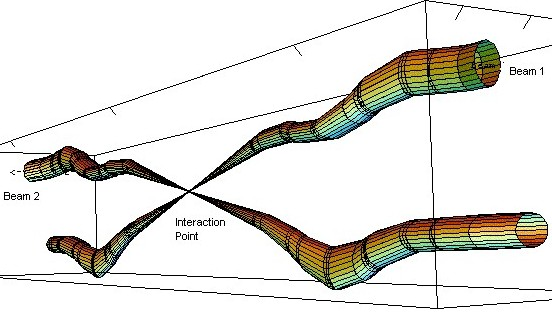
\includegraphics[width=0.6\textwidth]{plots/lhc/interactionpoint_lhc.jpg}
%    \caption{The geometrical configuration of beams leading up to the IPs at the LHC. Figure from \cite{LHC:beams}}
%    \label{fig:lhc_ip}
%\end{figure}
%Before protons reach the LHC, they are accelerated through the LHC injection chain which is comprised of the Proton Synchrotron (PS) and Super Proton Synchrotron (SPS). The PS accelerates protons to 25\GeV and provides them as packets with a 25ns spacing to the SPS. The SPS then accelerates the packets to an energy of 450\GeV. The acceleration of proton packets in the LHC itself is achieved through the radiofrequency (RF) system. The RF system is comprised of 16 RF cavities housed in 4 cryomodules located in LSS4 of the LHC ring. Each RF cavity delivers an oscillating longitudinal electric field of 5MV/m delivering an accelerating voltage of 2MV at a frequency of 400MHz. The RF cavities serve two primary purposes, first to accelerate the protons with every pass of the RF system, and second to group the packets of  protons from the PS into even tighter bunches to ensure a high luminosity at the collision points. The grouping into tight bunches happens because the protons tend to oscillate around those synchronised with the RF frequency. The proton injection is timed such that the center of a packet of protons is located just after the oscillating field maximum. Hence protons just before the maximum will accelerate towards the center, and protons after the maximum will decelerate towards the center, creating stable bunches. The number of possible stable bunches ($h$) is therefore equal to the number of possible synchronised protons. A proton is synchronised if the RF frequency is an integer multiple of the revolution frequency:
%\begin{equation}
%    f_{\text{RF}}=h\times f_{\text{rev}},\hspace{5pt} h=\frac{f_{\text{RF}}}{f_{\text{ref}}}.
%\end{equation}
%Substituting the protons revolution frequency of $c/27\text{km}$ and substituting the RF frequency of 400MHz, gives the value of $h\approx35640$, which is number of possible bunches. These are called RF buckets. Not every RF bucket is filled, and the number of occupied buckets in the LHC is 2808 \cite{LHC:design}\cite{LHC:acceleratorspedestrians}\cite{LHC:rfcavities}.
%only see the maximum accelerating voltage at the gap at an interval equal to an integer multiple of the 400MHz electric field frequency, and %Protons are initially injected into the cavities at an energy of 450\GeV after passing through the pre-accelerator known as the Super Proton Synchrotron (SPS). % Since there are 8 RF cavities, with every pass a proton receives 2MV$\times$8=16MeV of energy. Assuming protons travel at the speed of light, and taking the circumference of the LHC ring as 26669m, means that there are 11245 passes per second, resulting in $11245\times16\MeV=0.18\TeV$  %The RF cavities are responsible for bringing the beam energy up to 6.5 TeV (6.8TeV in run3). The frequency of the RF cavities is tuned to around 400MHz, 
%Now include some info about number of bunch crossings/second, number of interactions per second, primary verticles vs pileup vertices, etc.

\subsection{Detector Luminosity}\label{sec:lumi}

%The number of scattering events $N$ in a given amount of time is called the event rate, and depends on the geometric nature of the beam, and on the individual $pp$ interactions. For a given bunch crossing, each proton has an associated cross-sectional area where if another proton is within this, they may interact. It follows that the scattering probability is related to a quantity with units of area known as the \textit{scattering cross-section}, $\sigma$. $N$ is directly related to $\sigma$ and must satisfy
%\begin{equation}\label{eq:instlumi}
%    \frac{\mathrm{d}N}{\mathrm{d}t}=\mathcal{L}(t)\sigma,
%\end{equation}
%which defines the quantity known as the \textit{instantaneous luminosity} $\mathcal{L}(t)$.
%Integrating Equation \ref{eq:instlumi} yields the integrated luminosity $L$
%\begin{equation}
%    L=\int_{0}^{T}\mathcal{L}\mathrm{d}t,
%\end{equation}
%which is a measure of how much data has been taken in time $T$. Equation \ref{eq:instlumi} can be written in terms of $L$ as \cite{Buckley:PCP}
%\begin{equation}
%    N=\sigma L.
%\end{equation}
The instantaneous luminosity (Equation \ref{eq:instlumi}) depends on a number of beam parameters, and is given by
\begin{equation} \label{eq:lumi_1}
    \mathcal{L}(t)=\frac{N_b^2n_bf_{rev}\gamma_r}{4\pi\epsilon_n\beta^*},
\end{equation}
where $N_b$ is the number of particles per bunch, $n_b$ the number of bunches per beam, $f_{\text{rev}}$ the revolution frequency, $\gamma_r$ the relativistic gamma factor, $\epsilon_n$ the normalized transverse beam emittance (this reflects the beam quality, and is roughly defined as the smallest opening the beam can be squeezed through), $\beta^*$ the beta function (the width of the beam, squared, divided by the emittance) at the collision point and $F$ a geometric luminosity reduction factor. The linear dependence on $\gamma_r$ and square dependence on $N_b$ implies that a large luminosity requires beams of high energy and high intensity. Separate dipole magnetic fields and vacuum systems are required for the two beams, as both beams contain positively charged protons. At the IRs the two beams share a common 126m (for ATLAS and CMS) long beam pipe.

Integrating Equation \ref{eq:instlumi} yields the integrated luminosity $L$
\begin{equation}
    L=\int_{0}^{T}\mathcal{L}\mathrm{d}t,
\end{equation}
which is a measure of how much data has been taken in time $T$. Equation \ref{eq:instlumi} can be written in terms of $L$ as
\begin{equation}
    N=\sigma L.
\end{equation}

The luminosity in the LHC is not constant over a physics run. The beam intensities and emittances of the circulating beams degrade primarily due to the collisions themselves, leading to a decay in the luminosity. This is quantified with the luminosity lifetime, $\tau_L$. 

The expected integrated luminosity of the LHC of a luminosity run is given by
\begin{equation}
    L=L_0\tau_L(1-e^{-T_{\text{run}}/\tau_L}),
\end{equation}
where the assumption is made that the time for beam injection, ramping up the beam energy, ramping down the magnets, and programmed main systems checks total a turnaround time of $T_{\text{turnaround}}\approx 70\text{min}$. Assuming that the LHC is taking data 200 days a year for an optimum run time of 12h, the total maximum luminosity per year is about 120\invfb \cite{LHC:design}.

The Run-2 total integrated luminosity is shown in Figure \ref{fig:LHC:intlumi}. The Run-2 integrated luminosity recorded by ATLAS with good data quality is $140.1\infb$ \cite{LHC:atlaslumi}.

\begin{figure}[t]
    \centering
    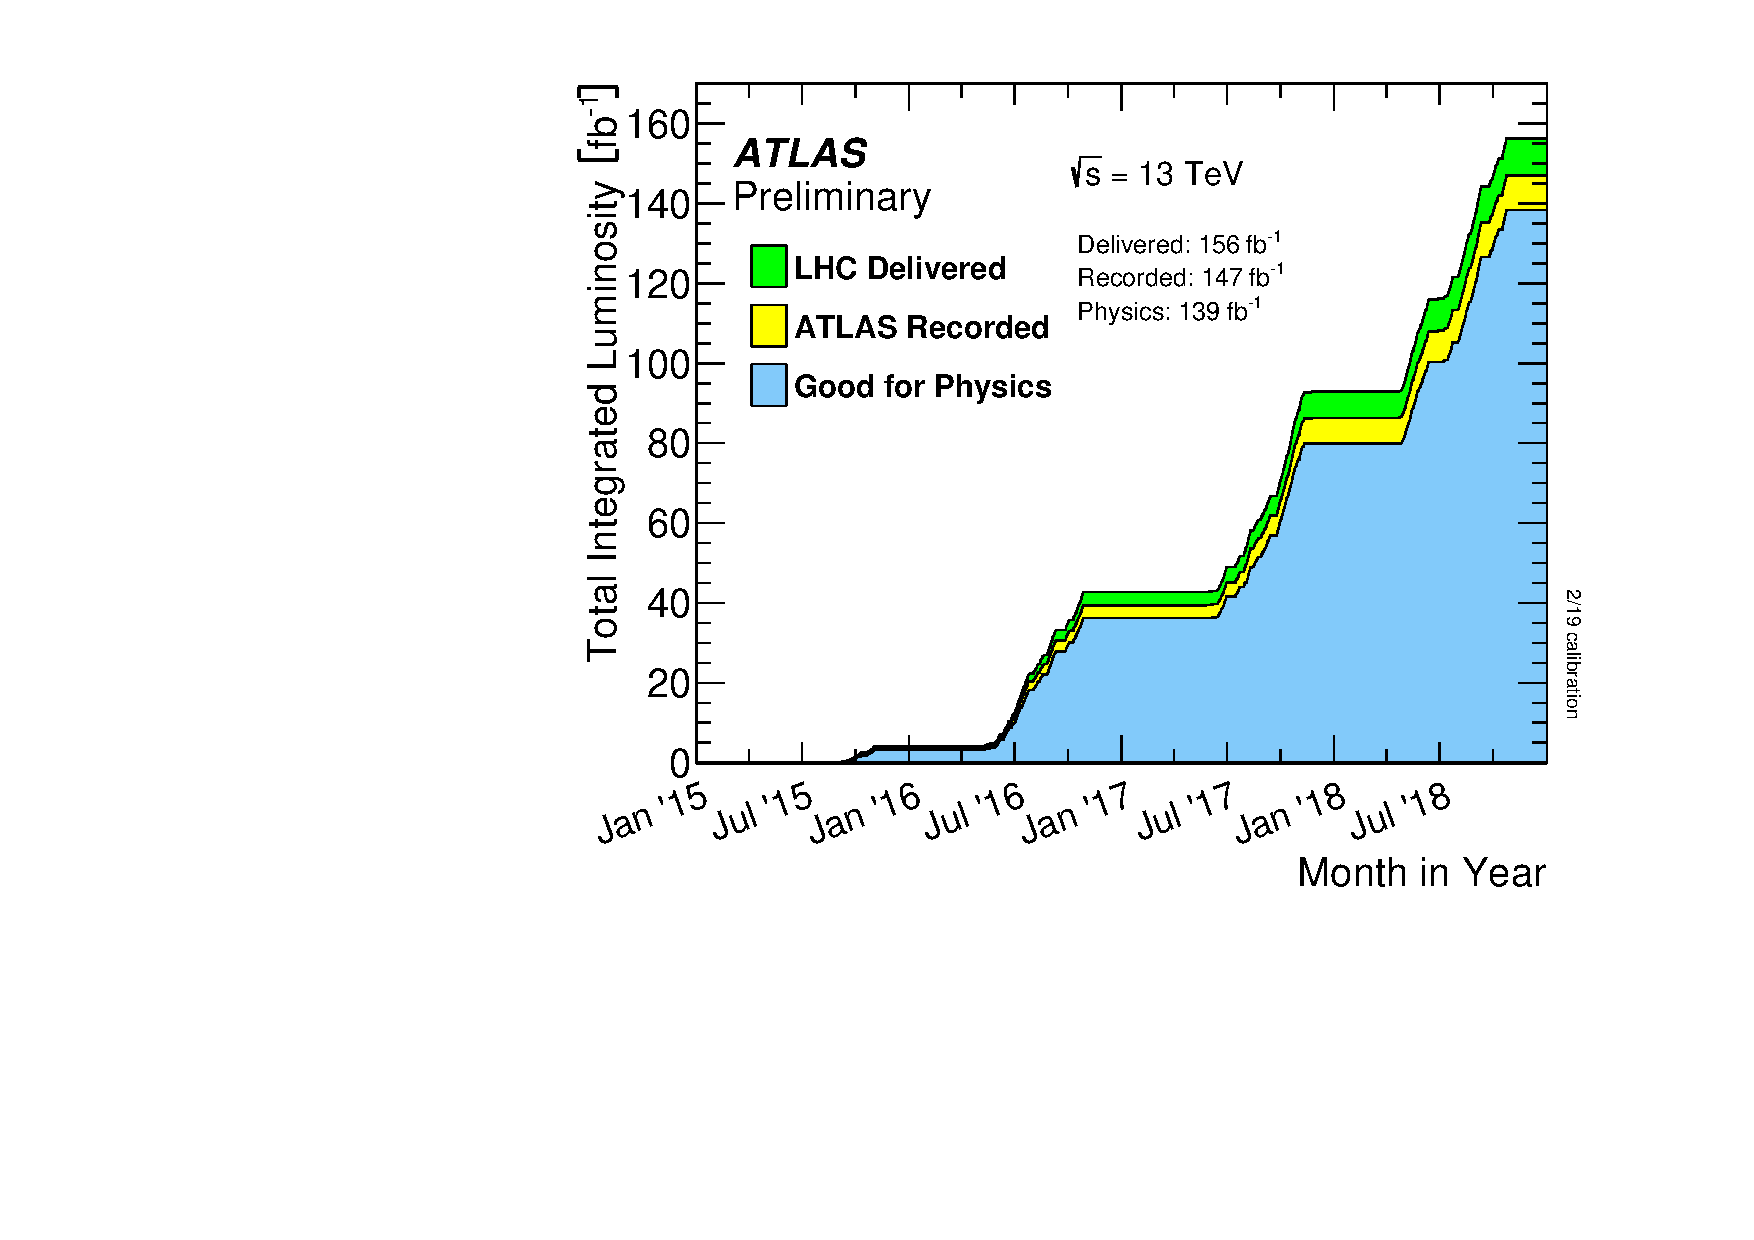
\includegraphics[width=\textwidth]{plots/lhc/intlumivstimeRun2DQall.pdf}
    \caption{The total integrated luminosity for Run-2 versus time. The green curve shows the luminosity delivered to ATLAS by the LHC. The yellow curve shows the luminosity recorded by ATLAS. The blue curve shows the luminosity of the dataset certified to be good data quality. Since this plot has been produced, the most accurate assessment of the total integrated luminosity certified good for physics has been updated to 140\infb \cite{LHC:atlaslumi}. Figure from \cite{LHC:deliveredlumi}.\label{fig:LHC:intlumi}}
\end{figure}

\subsection{Pile-up}

All LHC analyses need to contend with the harsh experimental conditions which come about due to the very large number of interactions per bunch crossing. The mean number of interactions per bunch-crossing (averaged over luminosity) $\langle\mu\rangle$ in Run-2 was $\langle\mu\rangle = 33.7$. The largest momentum transfer happens in the primary hard scatter interaction, all other secondary interactions are referred to as pile-up interactions and consist mainly of soft-QCD processes. There are two types of pile-up. In-time pileup refers to $pp$ collisions from the same bunch-crossing as the interaction of interest, whereas out-of-time pileup refers to $pp$ collisions occurring in bunch-crossings just before and after the interaction of interest. 

Pileup is responsible for a large number of soft hadrons distributed throughout the detector. Therefore the reconstruction of jets and Missing Transverse Energy (MET) are especially effected. Without pileup mitigation techniques, the energies of jets will in general be overestimated, and spurious jets not associated with the hard scatter will be included in the event leading to changes in the MET measurement. In addition to these biases, pileup also results in the degradation of the resolution of reconstructed quantities. The reason for this is that the pileup activity itself is not a fixed quantity, which therefore results in fluctuations of the bias due to pileup. The challenges associated with pileup in the context of object reconstruction is discussed in more detail in Section \ref{sec:objreco} \cite{Buckley:PCP,LHC:pileup}.

\section{The ATLAS Experiment}
The design of the ATLAS detector was initially motivated by the search for the Higgs boson and physics beyond the Standard Model (SM). The challenging experimental conditions at the LHC require fast, radiation-hard electronics and sensors. Large particle fluxes require a good detector granularity. An almost $4\pi$ acceptance is necessary to access the rich physics contained in the forward regions, such as the Vector Boson Scattering (VBS) process targeted in this thesis. Excellent electromagnetic (EM) calorimetry is a requirement for accurate electron and photon identification. The need for accurate jet and MET reconstruction dictates the energy resolution requirements for the hadronic calorimeter systems. Muon identification and momentum resolution must be able to determine the charge of high transverse momentum muons. Finally, a highly efficient trigger and data acquisition system is required to be able to select signal events on interest whilst rejecting backgrounds. 

Figure \ref{fig:atlas_detector} shows the different nested subsystems of the ATLAS detector. From the IP, the products of inelastic p-p collisions travel outwards through the detector subsystems. The origin of the coordinate system is defined as the IP. The beam direction defines the $z$-axis, whereas the $x-y$ plane is transverse to the beam direction. The positive $x$-axis points from the IP to the LHC ring centre, and the positive $y$-axis points upwards. The azimuthal angle $\phi$ is measured around the beam axis; and the polar angle $\theta$ is the angle from the beam axis. The rapidity is defined (in natural units) as
\begin{equation}
y = 1/2\ln [(E+p_z)/(E-p_z)], 
\end{equation}
where $E$ is the energy, and $p_z$ is longitudinal component of the momentum $\mathbf{p}$. In the $|\mathbf{p}|\gg m$ limit, the rapidity can be approximated by the pseudorapidity, $\eta=-\ln\tan (\theta/2)$. The distance between two particles $i$ and $j$ can be quantified using a metric, $\Delta R_{ij}$, which combines the rapidity separation $\Delta y_{ij}\equiv|y_i-y_j|$ and the azimuthal separation $\Delta \phi_{ij}\equiv|\phi_i-\phi_j|$
\begin{equation}
    \Delta R_{ij}=\sqrt{\Delta y_{ij}^2+\Delta\phi_{ij}^2},\hspace{25pt} \Delta R^{\eta}_{ij}=\sqrt{\Delta\eta_{ij}^2+\Delta\phi_{ij}^2}.
\end{equation}
The coordinate system used to describe the kinematics of particles detected at the ATLAS detector is represented schematically in Figure \ref{fig:atlas_coordinates}. The three-momentum of the final-state particle is denoted by $\vec{p}$. The transverse momentum, \pt, is defined by projecting $\vec{p}$ onto the $x-y$ plane and taking the magnitude. %The conservation of momentum in the transverse plane can be exploited due to the hermeticity of the ATLAS detector, and is used to define the missing transverse momentum, $\vec{p}_{T,{\text{miss}}}$, as the negative vector sum of the transverse momenta. The missing transverse energy, $E_T^{\text{miss}}$, or MET is given by the magnitude of $\vec{p}_{T,{\text{miss}}}$.
\begin{figure}[t]
    \centering
    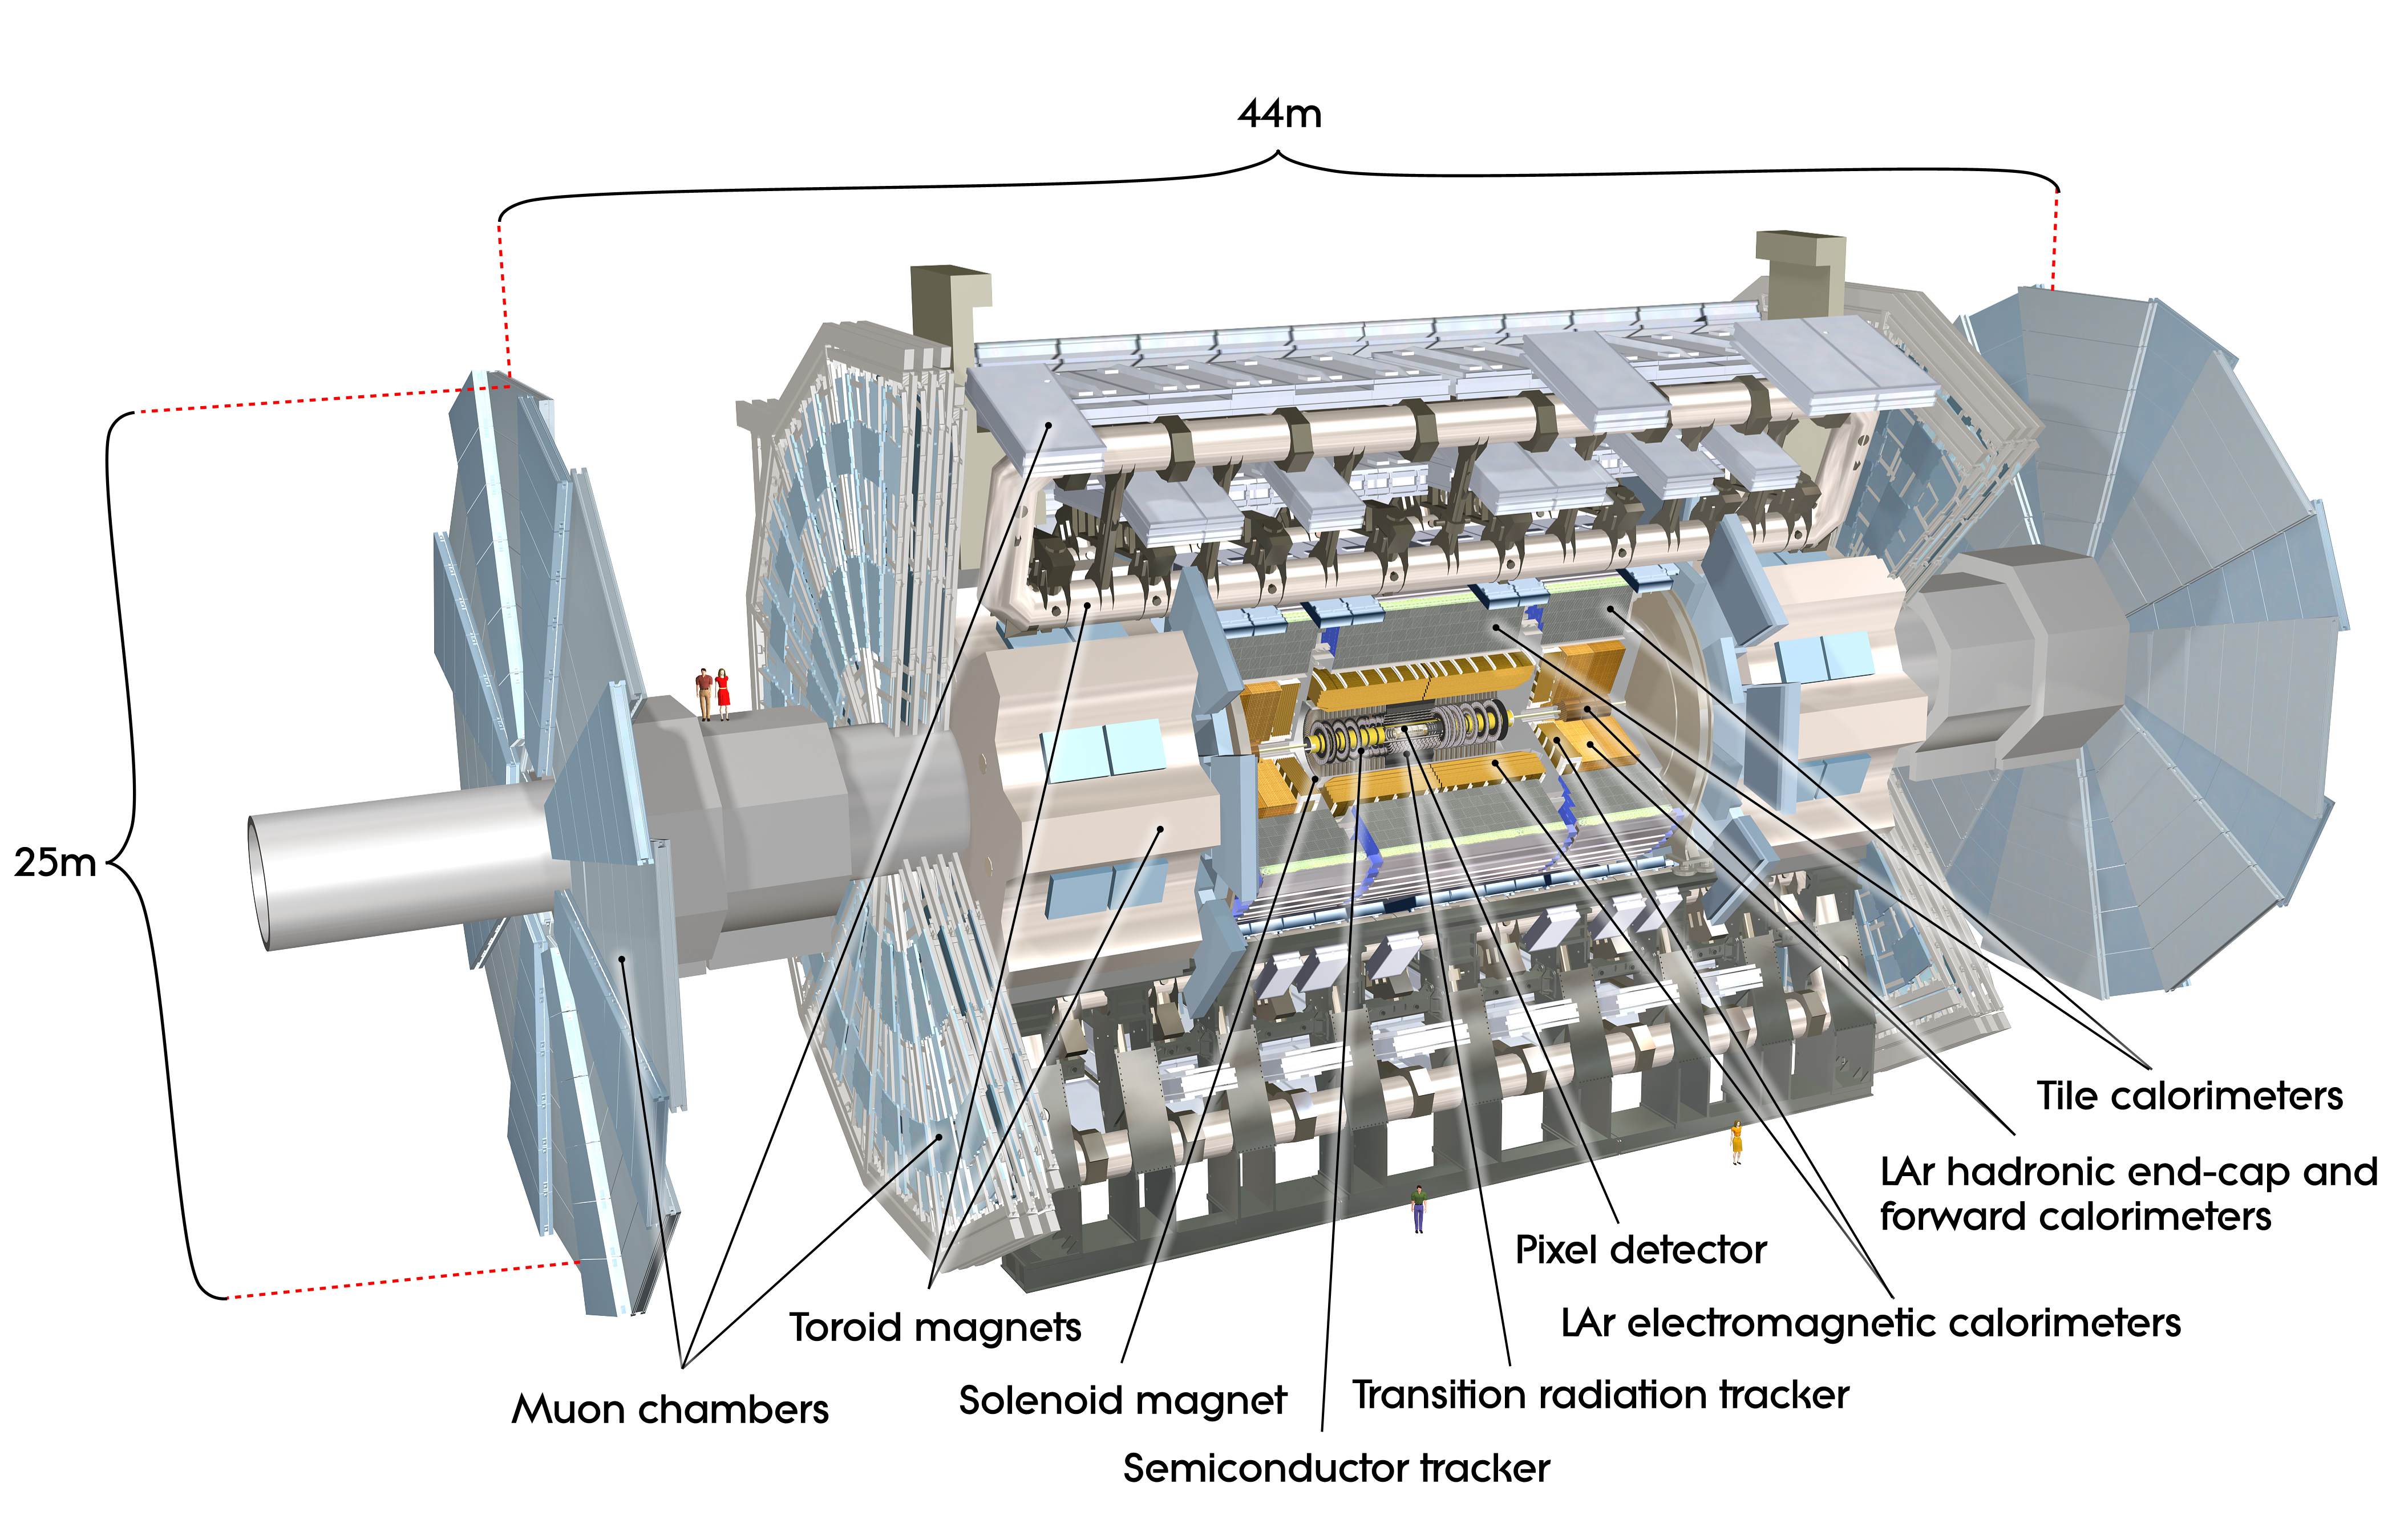
\includegraphics[width=\textwidth]{plots/atlas/ATLAS_Detector.jpg}
    \caption{A cut-out of the ATLAS detector showing the tracking, calorimeter, muon, and magnet systems. Figure from \cite{Atlas:detector}. \label{fig:atlas_detector} }
\end{figure}

\begin{figure}[t]
    \centering
    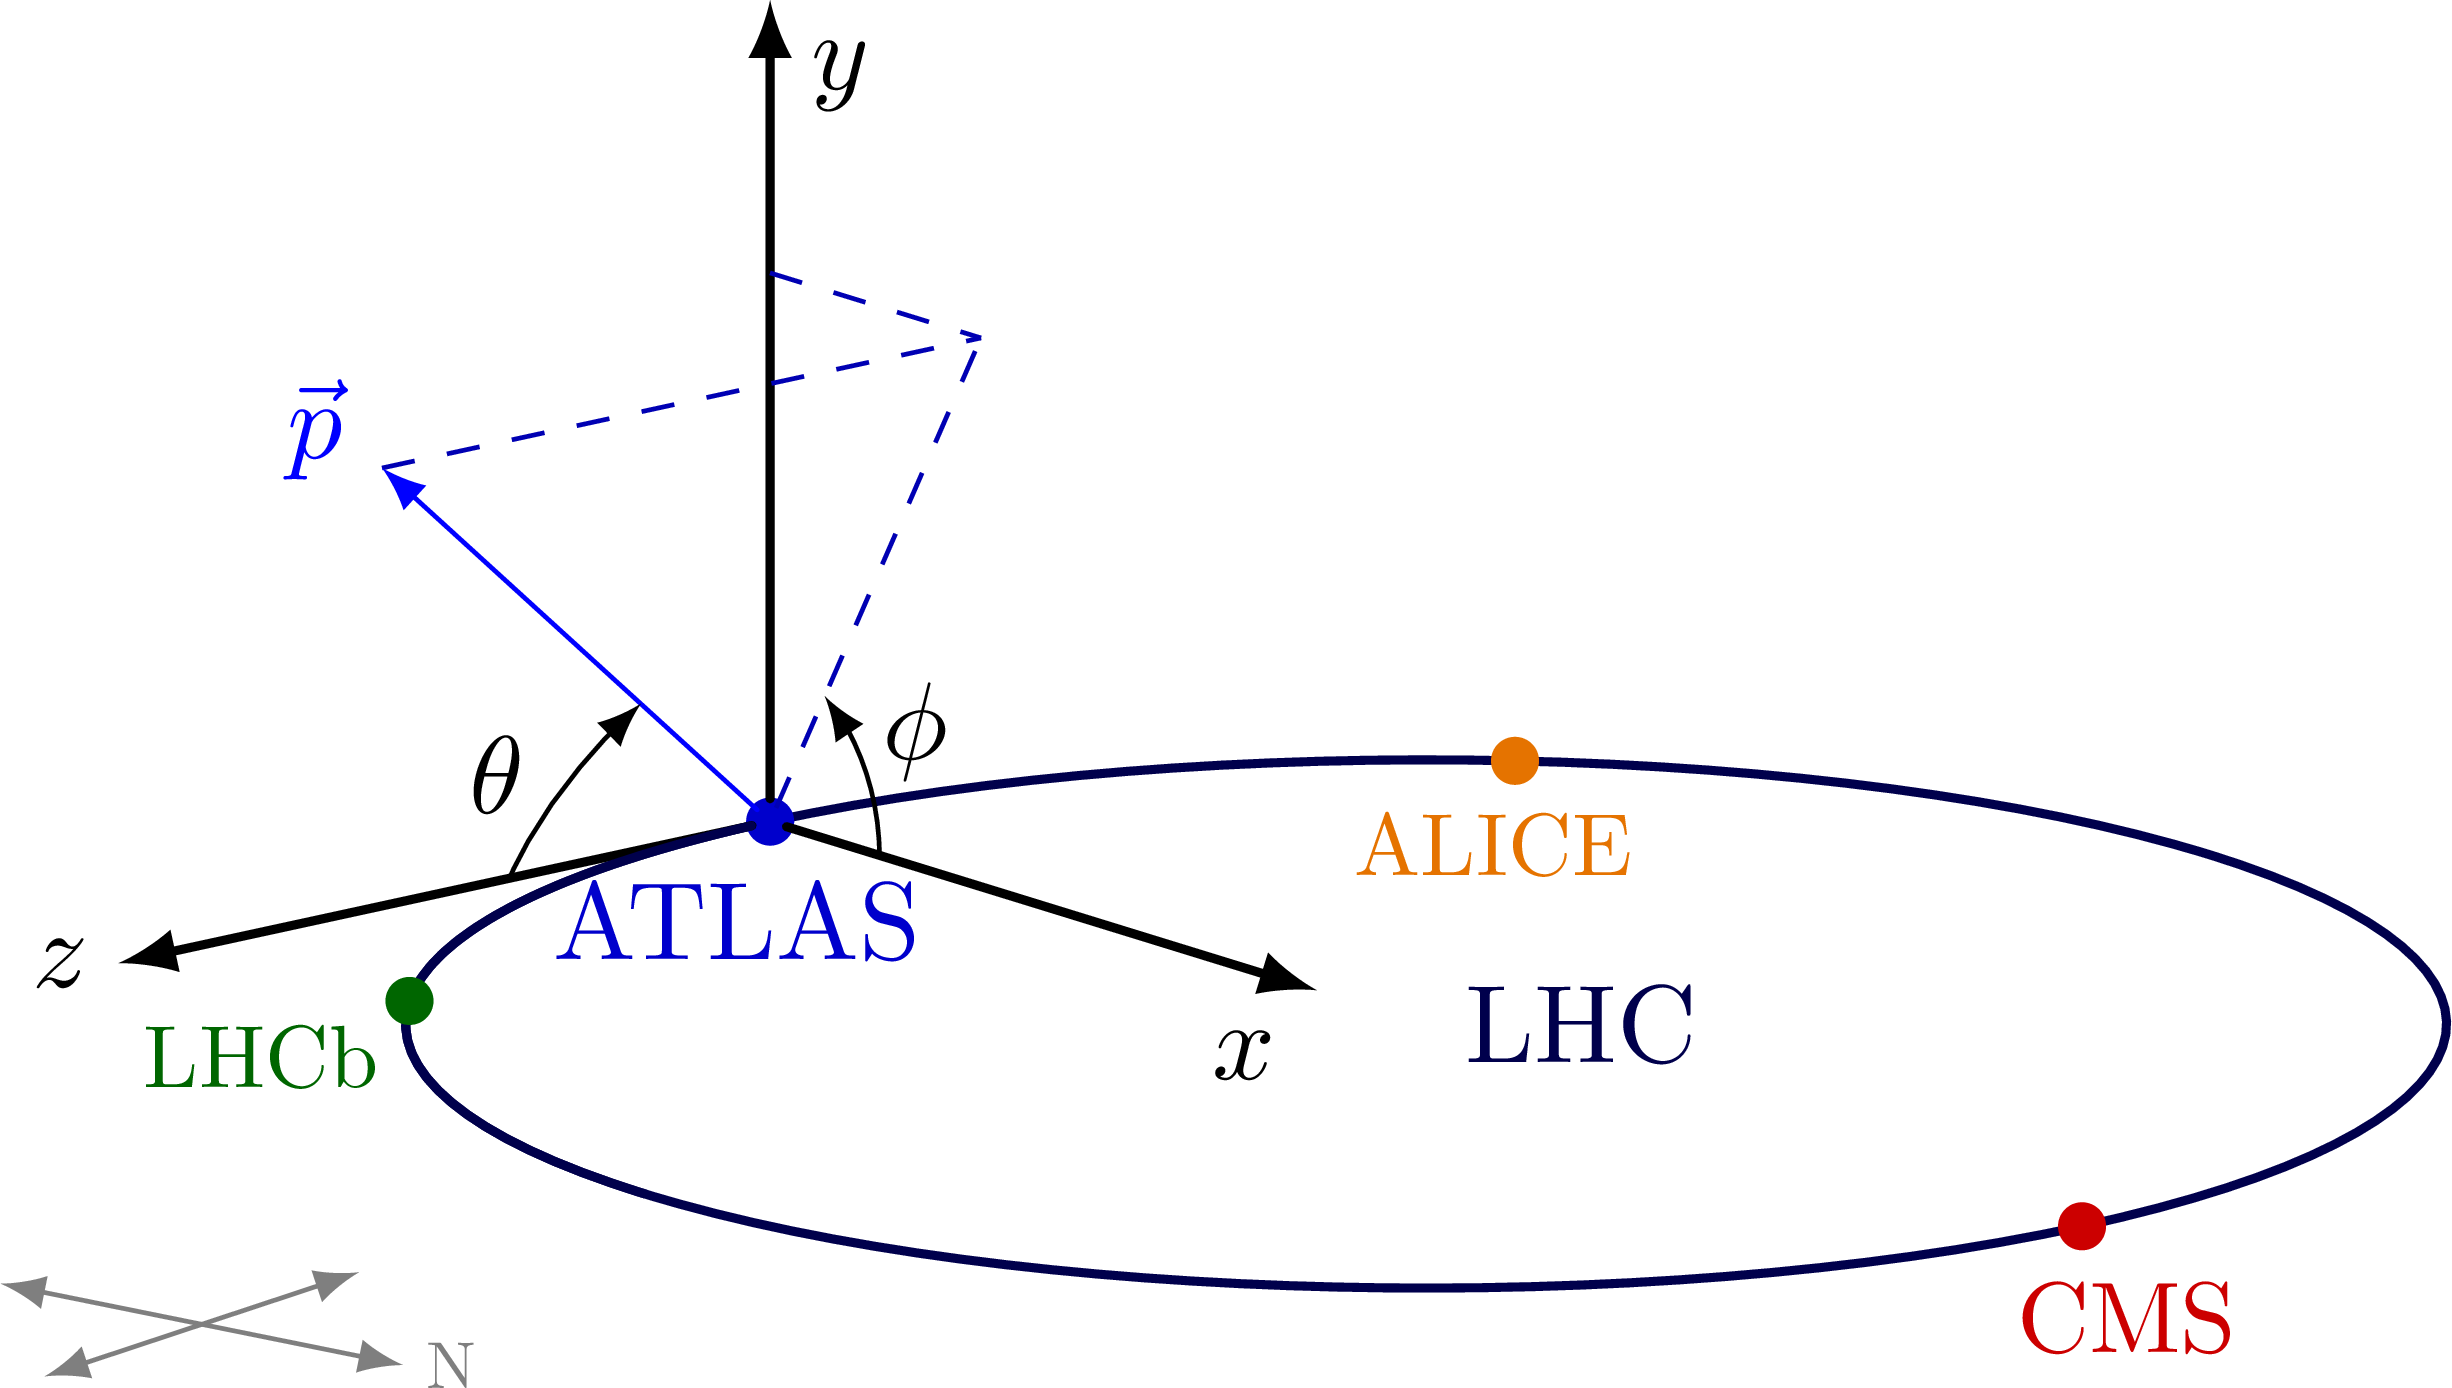
\includegraphics[width=0.7\textwidth]{plots/atlas/ATLAS_coordinates.png}
    \caption{The ATLAS coordinate system. Figure from \cite{Atlas:coordinates}.\label{fig:atlas_coordinates}}
\end{figure}

\subsection{Inner Detector}
The Inner Detector (ID) is comprised of three independent sub-detectors contained within a cylindrical envelope in a 2T solenoidal magnetic field. As charged particles travel through the ID, they ionise the material and leave behind a trail of electrical signals which are reconstructed to form tracks through the inner part of the ATLAS detector. The momentum can be inferred with high resolution from the curvature of the tracks. The ID also provides primary vertex (PV) and secondary vertex measurements (vertices are defined and discussed in Section \ref{sec:tracking}), and provides electron identification complimentary to the calorimeter. The ID covers the pseudorapidity range of $|\eta|<2.5$. In order of radial distance from the IP, the subdetectors consist of silicon pixel layers (Pixel detector), silicon microstrip layers (SCT detector), and layers of gaseous straw-tube elements called the Transition Radiation Tracker (TRT detector).  
%TODO: Mention insertable B-layer. See "Electron and photon energy calibration with the ATLAS detector using data collected in 2015" paper,
\subsubsection{The Pixel Detector}
At the inner radii, the highest resolution silicon sensors are required due to the difficulties in resolving tracks close to the IP. As such, the Pixel detector consists of three cylindrical silicon layers with individual sensor elements of $50\times400\mu\mathrm{m}^2$. The Pixel sensor elements are made up of 16 Front-End (FE) readout ASICS connected to a thin (250\microns) layer of silicon. When a charged particle travels through one of the pixel sensor elements, silicon atoms are ionised and liberated electrons travel through the bump bonds to the FE electronics. There are 2880 readout cells per FE ASICS chip. The readout cells of the FE amplify the sensor charge signal and compare it to a programmed discriminator threshold. For each readout, the hit pixel address, time stamp and amplitude information is transferred to buffers at the bottom of the FE.% Once the hit information is in the buffer, events are accepted depending the ATLAS Level-1 (L1) trigger decision, which happens every 2.5\microseconds. The transfer of the buffer content associated with one or more bunch-crossings is made to a readout driver (ROD) off the detector.

The top of the sensor elements contain a layer of kapton film onto which a Printed Circuit Board (PCB) is mounted containing a number of Surface Mounted Devices (SMDs) such as a temperature sensor, decoupling capacitors, and the Module Controller Chip (MCC). The MCC is responsible for Timing, Trigger and Control (TTC) logic tasks such as rejecting events where there are too many ($>15$) hits triggered in the FEs. The MCC is also responsible for extracting ordered hits from the FE and preparing them for transmission out of the pixel module \cite{Atlas:MCCmodule}.% A schematic view of a barrel pixel module is shown in Figure \ref{fig:atlas_pixelbarrelmodule} \cite{Atlas:MCCmodule}.
%\begin{figure}
%    \centering
%    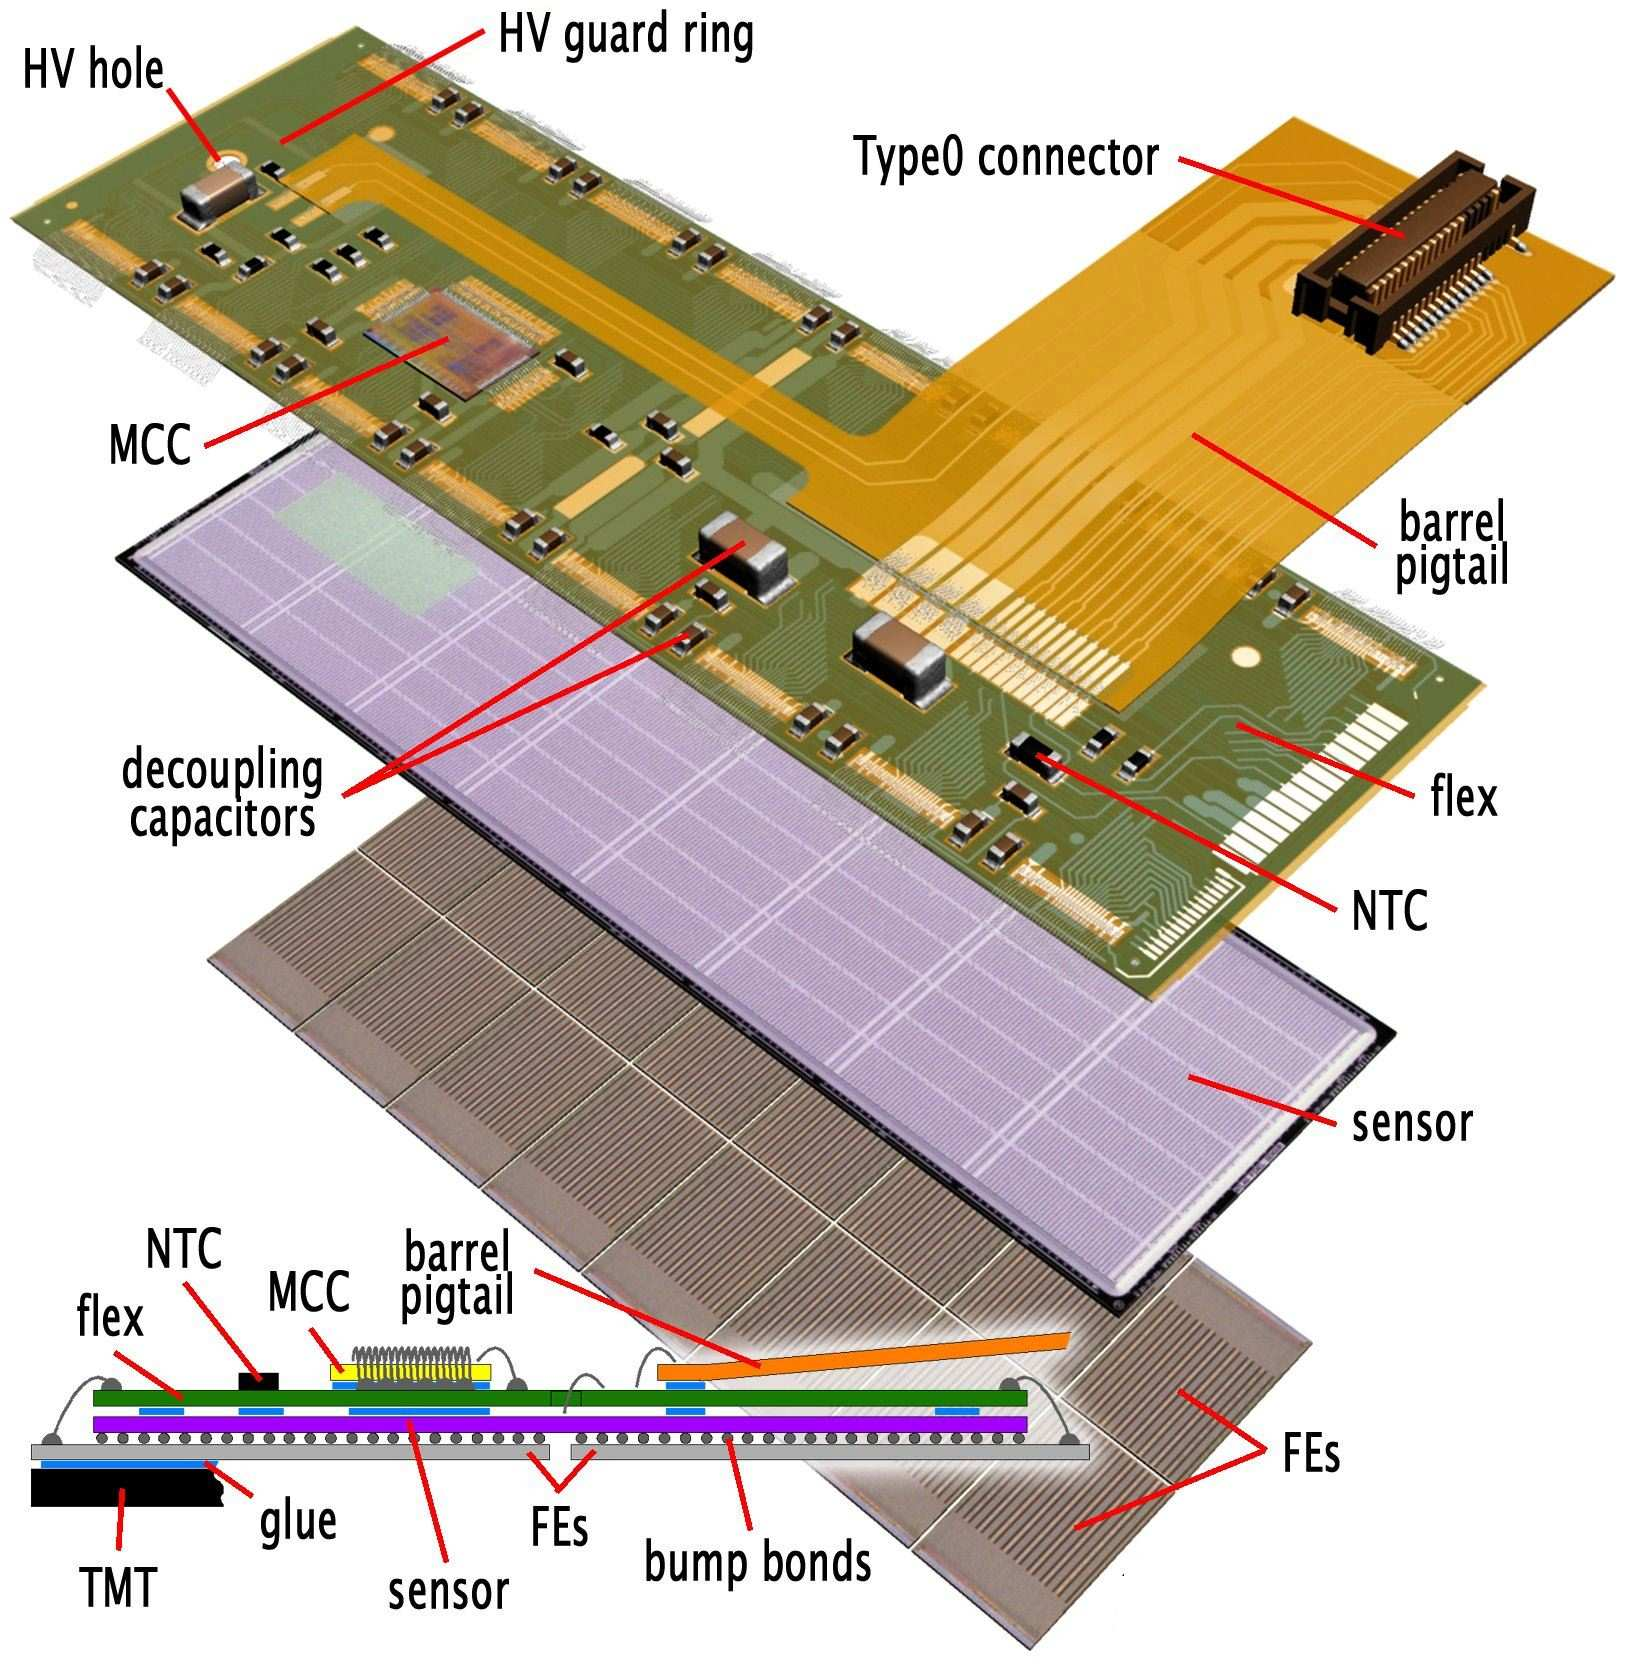
\includegraphics[width=0.5\textwidth]{plots/atlas/pixeldetectormodule.png}
%    \caption{A schematic diagram of one of the barrel pixel modules for the ATLAS ID system. In order of increasing radial distance from the beam, the FE ASICS, Si sensor tiles, and PCB with SMDs including the MCC are shown. A cross-section view of one of the barrel pixel modules is also shown.\label{fig:atlas_pixelbarrelmodule}}
%\end{figure}
%Remember to say something about radiation hardness (maybe operating temperature range?), and maybe something about the endcap modules maybe mention the spatial resolution ". At normal incidence, a spatial resolution of 12 µm is measured and approximately 80\% of the tracks have a single pixel hit. The resolution is not significantly degraded after irradiation. The optimal resolution of 4.7 µm (before) and 6.0 µm (after) irradiation is obtained for incident angles of 10–15deg (page 63 atlas design report) .
\subsubsection{The Semi-Conductor Tracker (SCT)}
The SCT enhances the high-resolution pattern recognition abilities of the ID at high radii, and consists of 4088 modules, arranged in four cylindrical layers in the barrel region and two end-caps, each containing nine disk layers. Each module consists of four sensors, with two sensors each on the top and the bottom side. A hybrid\footnote{Here, hybrid technology refers to the use of carbon-fibre substrates that have been directly interfaced with thin-film (polyamide) circuits to produce low-mass, thermally conductive, and radiation hard devices \cite{Atlas:Hybrids}} assembly bridges the sensors on each side. The top and bottom sensors are rotated through a relative ``stereo'' angle. In order to achieve the design azimuthal (the R-$\phi$ plane) and radial (R) resolutions of 17\microns and 580\microns respectively, the sensors are rotated at an angle of 40mrad. The silicon sensors are connected to binary signal readout chips.
%\begin{figure}
%    \centering
%    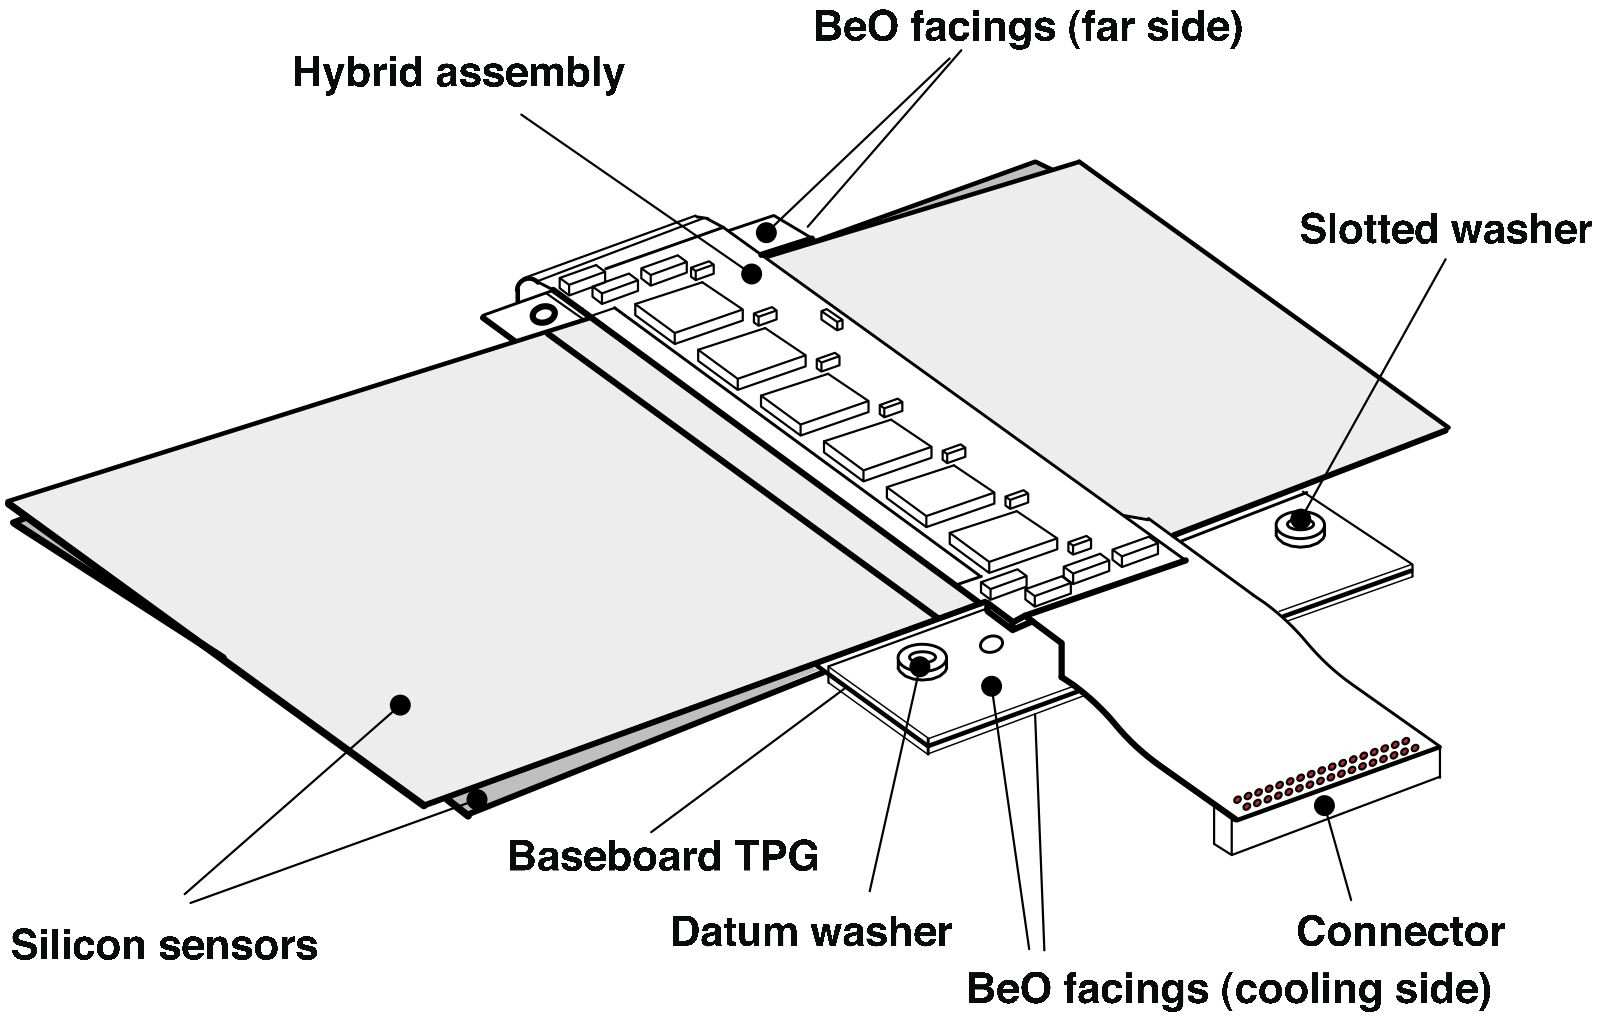
\includegraphics[width=0.75\textwidth]{plots/atlas/SCTmodule.png}
%    \caption{Drawing of a barrel SCT module. The Thermal Pyrolytic Graphite (TPG) material that comprises the baseboard conducts heat from the sensors to the octafluoropropane ($\mathrm{C}_3\mathrm{F}_8$) evaporative cooling system. The ceramic material Beryllia (BeO) is used on the surface layer of the TPG baseboard and is chosen due its high thermal conductivity and low density.\cite{Atlas:ThermalTechnologies} \label{fig:atlas_sctmodule}}
%\end{figure}
%The readout system for the SCT shares a number of common elements with the pixel and TRT. Namely, the same method of time-stamping, the use of buffers compatible with the L1 trigger latency, and the transfer to a ROD following an L1 trigger decision - note the ID is not part of the L1 trigger. The L1 trigger decision is made based on the calorimeters and muon detectors via the Central Trigger Processor (CTP). 
The readout hybrid on each SCT module contain 12 ASICs, with a total of 1536 readout channels. For each channel, there is a pre-amplifier, signal discriminator, and a shaper (splits each signal into overlapping channels, and applies a filter to optimise the signal/noise ratio). A buffer stores the hit information for approximately 3.2\microseconds, to allow for the L1 trigger decision (discussed in Section \ref{sec:ATLAS:trig}). 
\subsubsection{The Transition Radiation Tracker (TRT)}
The TRT enhances the performance of the ID at large radii, and consists of a barrel section and two end-cap sections. The basic elements of a TRT detector module are 4mm diameter polyimide straw tubes reinforced using carbon fibre bundles which stabilise the straw geometry by providing protection against environmental factors such as humidity and temperature. The straw tube walls are comprised of two multi-layer 35\microns thick films bonded back-to-back. Each tube contains a 31\microns diameter positively charged tungsten wire plated with 0.5-0.7\microns gold, directly connected to the front-end electronics. The tubes are filled with a mixture of 70\% Xe, 27\% C$\mathrm{O}_2$, and 3\% $\mathrm{O}_2$ gas. The gold plated wires act as anodes, attracting electrons liberated by charged particles and photons interacting with the gas mixture. The films contain a layer of aluminium, ensuring the sufficient electrical conductivity of the tube which acts as a cathode attracting positively charged ions \cite{Atlas:trt_designreport}.%next, put in citations, figure caption with all the explanation for the different elemtns of the film
%\begin{figure}
%    \centering
%    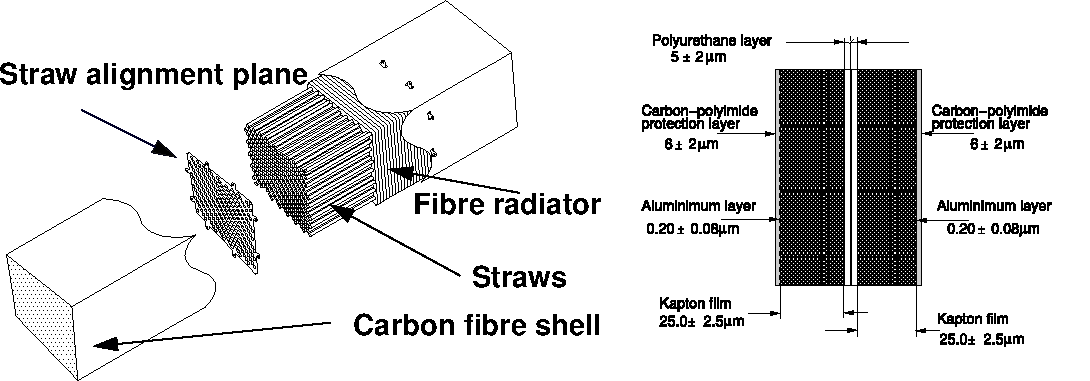
\includegraphics[width=\textwidth]{plots/atlas/trt.pdf}
%    \caption{Left, cut-out of one of the TRT barrel modules comprised of a carbon-fibre shell and polyimide straw tubes. Right, design of the (back-to-back) multi-layer film from which the straw tubes are manufactured. An aluminium layer on top of the kapton (polyimide) film enhances the electrical conductivity. The top carbon-polyimide layer protects the aluminium from damage from cathode etching effects. The polyurethane layer acts as a heat-activated adhesive and sealant. Figure adapted from \cite{Atlas:trt_module} and \cite{Atlas:trt_designreport}\label{fig:trt}.}
%\end{figure}
\subsection{Calorimeters}
%Two calorimeters - Tile and LAr. Full phi symmetry and coverage. Closest to beamline three cryostats - one barrel, two endcaps. Barrel: EM barrel calo, end cap cryostats: EM endcap calo; Hadronic EC calo; forward calo. Active detector medium is LAr, linear behaviour, stability of response over time, radiation hardness.
%
The ATLAS calorimetry system consists of electromagnetic (EM) and hadronic calorimeters. These are \textit{sampling} calorimeters, meaning that they are comprised of separate materials for inducing particle showers and for detecting the energy of the particles. Due to superior energy resolution, the energy measurements of most charged and neutral particles are provided by the calorimeters (rather than the tracking system). The electromagnetic calorimeters primarily make measurements of electrons and photons. The energy measurements of hadrons are primarily derived from signals in the hadronic calorimeter system.%The active media of the hadronic calorimeter system are scintellator sheets for the tile calorimeter and liquid Argon for the hadronic end-cap and forward calorimeters. Hadron energy losses occur primarily through nuclear interactions resulting in hadronic showers. 
%\newline
%Closest to the beamline, the calorimeters consist of sampling detectors with full $\phi$ coverage. These calorimeters are the electromagnetic barrel calorimeter, Electromagnetic End-cap Calorimeter (EMEC), Hadronic End-cap Calorimeter (HEC), and the Forward Calorimeter (FCAL). The detector medium for all these calorimeters is liquid Argon.
%\newline
\subsubsection{The EM Calorimeters}
The EM barrel and end-cap calorimeters have an accordion geometry and are comprised of lead and stainless-steel absorbers, LAr active material, and copper readout electrodes, which are positioned in the gaps between the absorbers. There are three active layers in the central region ($0 < |\eta| < 2.5$), and two in the forward regions $(2.5 < |\eta| < 3.2)$. The first layer is read out front, which is defined as the inner radius of the EM barrel, and the small-$z$ region of the end-cap. Conversely, the second and third layers are read out from the back. The barrel EM calorimeter is made up of two halves covering $|\eta|<1.475$. The cell granularity in $\Delta\eta\times\Delta\phi$ is $0.025/8\times0.1, 0.025\times0.025$, and $0.050\times0.025$ in the first, second, and third layers respectively, for $|\eta|<1.40$. In the $|\eta|>1.40$ region, the cell granularity is significantly coarser. The end-cap regions cover the $1.375<|\eta|<3.2$ range. The cell granularity in this region is the finest in the central part of the coverage range. The first layer has a granularity of $0.025/8\times0.1$ at $1.5<|\eta|<1.8$, and the granularity becomes coarser towards the limits of the end-cap coverage.  There is a crack region at $1.37<|\eta|<1.52$ where the transition between the barrel and end-cap calorimeters takes place. There is also a small crack at $|\eta|=0$ due to the fact that the calorimeter half-barrels are separated by 6mm at $z=0$.

When electrons and photons interact with the stainless-steel absorbers, narrow particle showers are produced as a result of a combination of bremsstrahlung, $e^{\pm}\rightarrow e^{\pm}\gamma$, and $\gamma\rightarrow e^+e^-$. Repeated interactions of the produced particles results in a cascade of particles with decreasing energy, which continues up until the pair production energy threshold. Below this threshold, photon energy losses occur primarily via compton scattering and the photo-electric effect, and the shower ceases. The characteristic amount of matter traversed by a particle before undergoing bremsstrahlung or pair production is the radiation length $X_0$, which is used to quantify the amount of material used in the calorimeter layers. The expectation values of the energies of the electrons $E(x)$ and intensity of the photons $I(x)$ in the shower follow exponential decay laws, with the decay constant determined by the radiation length
\begin{equation}
    \langle E(x)\rangle = E_0\mathrm{e}^{-\frac{x}{X0}},\hspace{20pt} \langle I(x)\rangle = I_0\mathrm{e}^{-\frac{7}{9}\frac{x}{X0}},
\end{equation}
where $x$ is the distance of the traversed material.
The EM calorimeters are complemented by pre-samplers which provide measurements of energy losses incurred by particles in the inner detector, i.e. before they interact with the calorimeter material.

\subsubsection{The Hadronic Calorimeters}

Hadrons interact with the nuclei of the absorbers via the strong force, resulting in the production of hadrons, especially pions. Each hadron undergoes additional interactions to form a cascade. Through nuclear de-excitation, lower energy neutrons, protons, $\alpha$-particles and photons are also produced. The hadronic shower also has a substantial electromagnetic component, which comes about primarily due to the decays of neutral pions \cite{Atlas:particleintmatter}. Hadronic showers are characterised by the nuclear interaction length $\lambda$, which is a function of the inelastic cross-section of the scattering process. Nuclear interaction lengths are typically an order of magnitude larger than radiation lengths, which explains why the ATLAS hadronic calorimeter system is larger than the EM calorimeter system \cite{Buckley:PCP}.

Hadronic showers represent a number of challenges. There are a considerable number of sources of energy leakage, such as backscattering and nuclear excitation processes, which do not result in an observable signal. In this way, the ATLAS calorimeter system is \textit{non-compensating}. This means that the calorimeter response (the ratio of the average calorimeter signal to the energy of the particle) is smaller for non-EM components of hadron showers than for EM components. Additionally, there are large fluctuations in the fraction of the EM and non-EM components of the larger hadronic shower. All of this degrades the hadronic energy resolution. 

The three hadronic calorimeters correspond to the Tile, the Hadronic End-Cap (HEC), and the Forward Calorimeters (FCal). The Tile calorimeter is comprised of an array of steel absorbers and scintillator sheets as the active medium. The Tile calorimeter comprises three layers, and covers the region $|\eta|<1.7$, behind the EM calorimeter, and has a radial depth of about $7.4\lambda$. The $\Delta\eta\times\Delta\phi$ cell granularity in the first two layers is $0.1\times0.1$, and $0.2\times0.1$ in the last layer. The scintillator signals are read out by photomultiplier tubes coupled to each tile edge through a series of fibres. The Tile calorimeter has a total of 187456 readout channels \cite{Atlas:design}.

The HEC calorimeter uses copper as the absorber and liquid-argon as the active material. The HEC comprises four layers, which cover the range $1.5 < |\eta| < 3.2$. The HEC calorimeter has a radial depth of about $9.7\lambda$. The $\Delta\eta\times\Delta\phi$ cell granularity is $0.1\times0.1$ at $1.5<|\eta|<2.5$, and $0.2\times0.2$ at $2.5<|\eta|<3.2$. The gaps between the plates that comprise the HEC modules contain the readout modules, which are made up of three electrodes separated by honeycomb spacers. The central electrodes contain readout cells of size $\Delta\eta\times\Delta\phi=0.1\times0.1$ in the $|\eta|<2.5$ region and $0.2\times0.2$ for larger values of $|\eta|$. The HEC calorimeter contains 5632 readout channels \cite{ATLAS:HEC,Atlas:design}.

The FCal extends the calorimeter coverage into the forward regions ($3.1 < |\eta| < 4.9$), and has a radial depth of about $10\lambda$. The FCal comprises one electromagnetic module (FCal1) and two hadronic modules (FCal2, FCal3). The $\Delta\eta\times\Delta\phi$ cell granularities are $3.0\times2.6, 3.3\times4.2$, and $5.4\times4.7$ in the central cells of the FCal1, FCal2, and FCal3, respectively, and the granularities are around four times finer around the coverage limits. Copper is used as the absorber for FCal1 to optimise the energy resolution of measurements of EM showers, and tungsten is used as the absorber in FCal2 and FCal3 to contain the lateral spread of hadronic showers. Each of the FCal modules contain readout electrodes which are connected to the module faces. Signals are read out from the side nearer to the interaction point for FCal1, and from the side furthest from the interaction point for FCal2 and FCal3. The FCal calorimeter contains 1762 readout channels \cite{Atlas:design}.

\subsubsection{Energy Resolution}
The energy resolution defines the most important attributes of the ATLAS calorimeter system and is often quoted as follows
%
\begin{equation}
    \label{eq:energyres}
    \frac{\sigma(E)}{E}=\frac{a}{\sqrt{E}}\oplus\frac{b}{E}\oplus c\%,
\end{equation}
%
where $\oplus$ denotes addition in quadrature. The $a$ term is the \textit{stochastic} term, which primarily arises due to fluctuations in the number of particles produced in the shower. This term limits the low-energy performance of the calorimeters. The $b$ term describes electronic noise primarily from readout electronics, and the $c$ term is a constant term which dominates in the high energy limit. Measurements of the calorimeter energy resolutions are made using lepton and hadron test-beams. Results from these measurements are shown in Figure \ref{fig:energyres}. Note that for the LAr energy resolutions results using electron test-beams are fitted with equation \ref{eq:energyres}, without the $\frac{b}{E}$ term. This is because a noise-subtraction step is implemented for every energy measurement since the noise here depends on the gain of the LAr calorimeter cells. The pion test-beam results for the combined calorimetry shown in Figure \ref{fig:energyres} utilises the full functional form of equation \ref{eq:energyres}. %Note that since the noise depends on the gain of the calorimeter cells (which is non-uniform with energy), for the LAr energy resolution measurements using lepton test beams, a noise-subtraction step in implemented for each energy point to obtain the intrinsic resolution of the calorimeter. Hence, for these measurements the energy resolution measurements after noise-subtraction are fitted using equation \ref{eq:energyres}, without the $\frac{b}{E}$ term.

\begin{figure}[t]
    \begin{minipage}{6in}
        \centering
        \raisebox{-0.5\height}{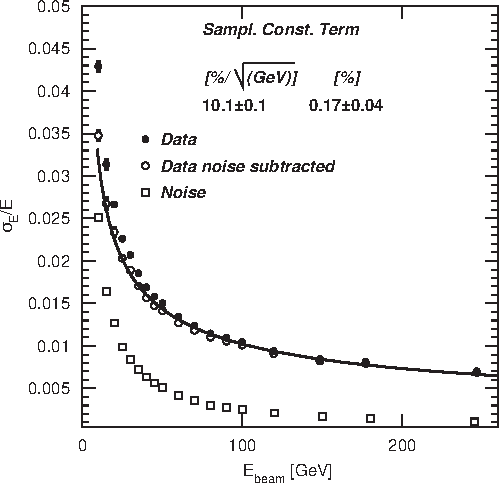
\includegraphics[width=0.40\textwidth]{plots/atlas/energy_resolution.pdf}}
        \hspace*{.2in}
        \raisebox{-0.5\height}{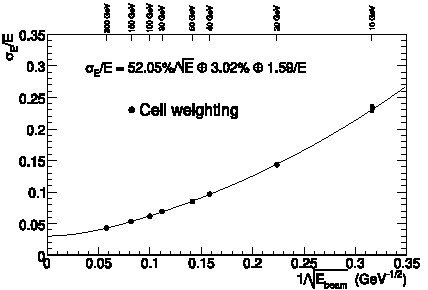
\includegraphics[width=0.53\textwidth]{plots/atlas/pion_energy_resolution_LAR_TILE.pdf}}
        \centering
    \end{minipage}
    \caption{Fractional energy resolution in the ATLAS EM barrel calorimeter as a function of the beam energy obtained from electron test-beams at $|\eta| = 0.687$ (left). Fractional energy resolution obtained using pion test beams for combined LAr and tile calorimetry at $|\eta|=0.25$ (right). The energy resolution for pion test-beams is shown as a function of $1/\sqrt{E_{\text{beam}}}$. Markers corresponding to $E_{\text{beam}}$ are shown at the top of this plot for the ease of comparison. 100$\GeV$ electrons have an energy resolution of about $1.1\%$ in the central region of the calorimeter system, compared to about $6.2\%$ for hadrons. Note that in regions where the forward calorimetry (FCal) system is in use ($3.1 < |\eta| < 4.9$), the energy resolution increases to about 5$\%$ for 100\GeV electrons, and to about $8\%$ for $100\GeV$ pion test-beams \cite{Atlas:EMCalo,Atlas:design}.\label{fig:energyres}}
\end{figure}

\subsection{Muon Spectrometer}

The muon spectrometer (MS) covers the pseudorapidity range of $|\eta|<2.7$. The MS measures charged particles (primarily muons) that penetrate the barrel and end-cap calorimeters. The primary purpose of the MS is to identify and measure high momentum muons. The MS is designed to measure the transverse momentum of muons with $\pt>1\TeV$ to an accuracy of $10\%$. The MS is also capable of triggering on muon tracks, and is designed to trigger in the region of $|\eta|<2.4$. The precision momentum measurements of the MS system are provided by Monitored Drift Tube (MDT) chambers and Cathode-Strip Chambers (CSC). This is complemented by Resistive Place Chambers (RPC) and Thin Gap Chambers (TGC) which provide fast triggering capabilities to clarify events of interest. 

The MS is partitioned in the barrel and endcap regions into three layers referred to as the inner, middle, and outer layers. Two MDT chambers are housed in each of the layers. There are a total of twelve MDT segments in radially consecutive stations (collection of segments in a layer) spanning three layers. The CSCs are located in the inner endcap layer. Both the CSCs and MDTs are segmented into large and small chambers. The RPC system is layered into three trigger stations and is comprised of large and small small segments. The RPCs are located in the middle and outer layers of the barrel. The TGC system is comprised of seven layers in the EM layer, and two layers in the inner endcap layer.
%\begin{figure}
%    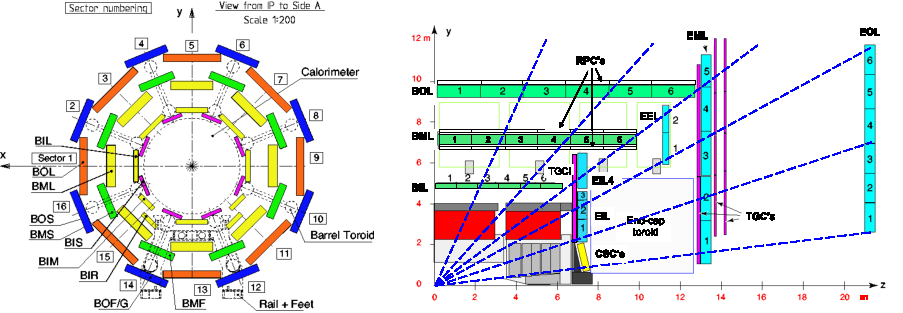
\includegraphics[width=\textwidth]{plots/atlas/ms.pdf}
%    \caption{Cross-sections of the barrel muon system perpendicular to the beam axis (left), and in the bending plane containing the beam axis (right). In the right figure, the blue dashed lines represent muon trajectories in the absence of a magnetic field. Figure from \cite{Atlas:design}. \label{fig:ms}}
%\end{figure}
%\newline

The MDTs cover the pseudorapidity range of $|\eta|<2.7$ in all but the inner most layer. The MDTs are drift tubes with a diameter of about 3cm, and are pressurised with a mixture of Ar and $\text{CO}_2$ gas. The centers of the tubes contain a $50\mu m$ diameter tungsten-rhenium wire. When a charged particle enters the tube, the gas is ionised, and liberated electrons drift to the wire and the ions drift to the walls of the tube. 

The MDTs provide a position resolution of $80\microns$. The position measurements are determined by the drift time of the charges deposited in the MDTs. Muon tracks are reconstructed using these measurements, and this is discussed in more detail in Section \ref{sec:muon}. The $\pt$ of the muon is directly inferred from the radius of curvature of the tracks. For the required momentum resolution, a sagitta \footnote{The perpendicular distance between the apex of the arc of the track, and the chord intersecting the inner and outer layers of the MDT.} along $z$ of about $500\mu m$ needs to be known with a resolution better than $50\mu m$.  

The CSC system covers the forward $2<|\eta|<2.7$ region. The CSC system are two disks of eight wire chambers. Each chamber is filled with an Ar$\text{CO}_2$ gas mixture and contains an array of high voltage anode wires and cathode planes at ground potential. Precision position measurements in both $R$ and $z$ are obtained with a resolution of $60\mu m$ via measurements of the charge distributions on the cathodes.

The muon trigger system consists of RPCs and TGCs. The RPCs are used in the barrel region ($|\eta|\leq 1.05$), and TGCs in the  end-cap region ($1.05\leq|\eta|\leq 2.4$). Different technologies are used in different regions due to different requirements on spatial and timing resolution as well as considerations of trigger rate. The RPCs are gaseous parallel electrode-plate detectors. These are comprised of two parallel dielectric plates separated by 2mm. In the 2mm gap is a gas mixture, and a high electric field is applied (4kV/mm) between the plates. When a charged particle travels through the gas gap, the gas is ionised, and the positive ions travel towards the cathode, and the electrons towards the anode. The liberated electrons are accelerated by the high electric field to a sufficient extent such that they go on to liberate additional electrons from the gas medium resulting in a chain reaction of ionisation events. This process is known as a Townsend avalanche \cite{ATLAS:townsend}. The electrical signals from the avalanches are read out via metallic strips mounted on the outer faces of the resistive dielectric plates. TGCs operate on the same principle as the wire chambers of the CPC. The primary function of the RPCs and TGCs are to facilitate triggering on muon events, but they also complement the MDT tracking data. Through the additional measurement of the track coordinates in the non-bending $\phi$ plane, which complement the measurement in the bending $\eta$ plane, the MDT and RPC (and TGC in the end-cap region) measurements can be combined in an unambiguous way \cite{Atlas:design,ATLAS:MS}.

\subsection{ATLAS Trigger and Data-acquisition\label{sec:ATLAS:trig}}
The ATLAS trigger and data-acquisition (TDAQ) system is responsible for deciding which events from of the $\num{40e6}$ bunch-crossings per second at the ATLAS interaction point to save for physics analyses, calibrations, monitoring, and performance measurements. The trigger system is comprised of two stages. These are the Level-1 (L1) and HLT triggers. 

The hardware based Level-1 trigger is principally responsible for making the trigger decision to reduce the event rate from 400MHz to maximally 100kHz by processing signals from the calorimeters and MS. The L1 trigger consists of the L1Calo, L1Muon, L1Topo, and Central Trigger subsystems. The L1Calo comprises the Cluster Processor (CP) and Jet/Energy-sum Processor (JEP), which receive calibrated calorimeter signals in parallel to identify physics object candidates. Tile calorimeter and MS information is passed to the L1Muon, where searches are performed for signals consistent with muons originating from the interaction point. The L1Topo receives object candidates from the L1Calo and L1Muon in order to reconstruct topological observables such as invariant masses and angular observables. The outputs from the L1Calo, L1Muon and L1Topo are processed by the Central Trigger Processer (CTP) which makes the L1 trigger decision. The CTP is also responsible for applying a preventative \textit{dead-time} mechanism to moderate the L1 accept rate. For every L1 trigger decision, ``Regions Of Interest'' (RoIs) are identified using $\eta$ and $\phi$ information \cite{Buckley:PCP,Atlas:tdaq,Atlas:willL1Trigger}. 

After a L1 trigger accept, the events are processed by the software-based High-Level Trigger (HLT). Events processed by the HLT use fine-granularity calorimeter and precision MS information, as well as tracking information from the ID. The HLT performs the event reconstruction within the L1 RoIs or the full detector, as needed. In most cases, the HLT performs a fast first-pass reconstruction using a sequence of \textit{feature-extraction} algorithms. A trigger decision is then subsequently made by the \textit{hypothesis} algorithms. Afterwards, more precise and computationally expensive algorithms reconstruct high level physics objects in greater detail -- this is called the \textit{online reconstruction}. The online reconstruction of objects is less precise, but nevertheless similar to the offline reconstruction (Section \ref{sec:objreco}). Events passing the HLT decision are saved to the CERN Tier-0 computer centre for offline reconstruction, this occurred at a rate of approximately 1.2kHz during the 2018 data taking for Run-2 for triggers dedicated to physics analyses \cite{Atlas:tdaq,Atlas:trig2015}. 

Each combination of L1 and HLT event selections has an associated set of \textit{prescale} factors, which take values of at least 1. A prescale value of $n$ means that an event has probability of $1/n$ of being kept. Prescales are defined for both L1 and HLT, but the prescale is implemented slightly differently in each case. For L1 prescales, since the CTP is fast, the trigger decision is still computed for every event, but for each event that passes the trigger decision, a random number generator determines whether it is passed to the HLT. Since the online reconstruction is expensive, HLT prescales are applied before the trigger decision is computed. The reason for applying prescales is to prevent saturating the allowed bandwidth. This is possible for certain processes, such as minimum bias, which have very loose triggers and therefore very high event rates \cite{Buckley:PCP}.

A combination of L1 and HLT prescales and event selections comprises an item in the \textit{trigger menu}, which consists of a list of:
\begin{itemize}
    \item \textit{Primary} triggers: used for physics analyses, usually unprescaled.
    \item \textit{Support} triggers: used for monitering, performance, and efficiency measurements. These are usually prescaled, and have small HLT rates of around 0.5Hz
    \item \textit{Alternative} triggers: used in the commissioning of new triggers. These use alternative reconstruction algorithms, and are complimentary to primary triggers
    \item \textit{Backup} triggers: used in case CPU usage or output rate of primary triggers too high. These are similar to primary triggers but with tighter selections.
    \item \textit{Calibration} triggers: used for detector calibrations, and run at high rates. 
\end{itemize} 
All items in the trigger menu are connected to an HLT data stream. The \textit{Main} physics stream contains events for physics analyses, and a small fraction of these events are written to the \textit{Express} stream which is used to derive offline calibrations soon after data taking. There are about twenty additional streams for calibration, monitoring and detector performance studies in addition to specialised \textit{Trigger-Level Analysis} and \textit{debug} streams. The physics \textit{Main} stream events are partitioned into categories called trigger signatures, for example ``single leptons''. Each trigger signature is split up into multiple items giving the L1 and HLT trigger thresholds, object multiplicities, online object isolation requirements, as well as peak trigger rates. For example, for an offline selection of a single isolated muon with $\pt>27\GeV$, the corresponding trigger in the 2018 trigger menu corresponds to a 20\GeV single muon requirement at L1, a 26\GeV isolated muon at HLT, with a peak L1 trigger rate of 16kHz, and peak HLT trigger rate of 218kHz. The values of the offline \pt values in the trigger menu are usually defined as the value where the trigger efficiency\footnote{The trigger efficiency is the number of correctly identified objects divided by the actual number of objects above a certain \pt threshold. At the LHC, typically trigger efficiencies of $>90\%$ (10\% accuracy) are deemed acceptable \cite{Atlas:triggeratlhc}.} plateaus \cite{Atlas:trigmenu}.
%single lepton triggers
%Include a few sentances on how the online resonstruction differs from the offline

\subsubsection{Photon and Lepton Triggers}
%Mention figure for e/y trigger reco.  

Electron and photon candidate RoIs are identified in the L1 trigger using only calorimeter information in the central ($|\eta|<2.5$) region. The identification works by iterating over groups of EM calorimeter cells, called ``trigger towers'', of size $2\times2$ ($\Delta\eta\times\Delta\phi = 0.1\times0.1$). Within each $2\times2$ region, the \et of all the four possible $1\times2$ and $2\times1$ pairs of towers is calculated. If the maximum \et among these pairs passes the L1 \et threshold (nominally 22\GeV), the $2\times2$ region is identified as an RoI. An additional hadronic activity veto can be applied, where candidates are rejected if the $2\times2$ hadronic calorimeter trigger towers behind the EM cluster have an \et above a given threshold. An isolation requirement can also be defined by a threshold on the energy of the EM isolation ring around the $2\times2$ RoI. Figure \ref{fig:triggertower} shows a schematic view of the EM and hadronic trigger towers \cite{Atlas:trigegamma,Atlas:trig2015}.
\begin{figure}[t]
   \centering
   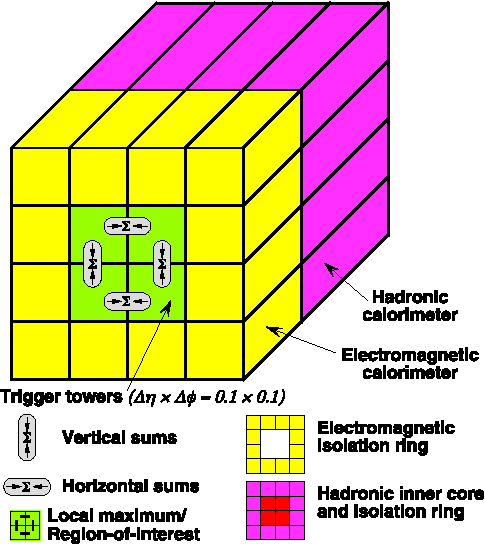
\includegraphics[width=0.6\textwidth]{plots/atlas/triggertower.pdf} 
   \caption{Layout of the trigger towers used in the L1 trigger electron and photon reconstruction. The EM calorimeter cells are colored in yellow, and the majenta cells denote the hadronic calorimeter cells. Figure from \cite{Atlas:trig2015}.\label{fig:triggertower}}
\end{figure}

 % The online-reconstruction differs in that the GSF refit is not performed for electron tracks, only topo-clusters are used (rather than variable-sized superclusters), and for the assessing of pileup, only information from the average number of interactions per bunch crossing, $\langle\mu\rangle$ is used, rather than the number of primary vertices. Additionally, some cell energy and pileup corrections are not implemented for the online-reconstruction. In the 2x2 central region of the towers, all possible 1x2 or 2x1 pairs of cell energies are summed, and if a predefined \et threshold is reached, the 2x2 region is flagged as a RoI.
The reconstruction of electrons and photons at the HLT is performed in each RoI identified by the L1 trigger. For the fast stage of the HLT decision, a cut-based algorithm is used for electrons below $15\GeV$ and for the reconstruction of all photons. Objects are identified based on the \et of the cluster and the shape of the EM shower. %The algorithm starts by reconstructing clusters in the L1 RoI. For speed, use only the second layer of the EM calorimeter is used (since electrons and photons deposit most energy in second layer) to find the ``pre-seed'' cell, which is the cell with the largest \et. Regions of the calorimeter around the preseed are searched for the seed, the local maximum. Electrons and photons are then reconstructed using $3\times7$ (barrel) and $5\times5$ (endcap) clusters. Corrections derived from offline reconstruction algorithms are applied to improve the cluster energy and position resolutions. The object identification is based on the \et of the cluster and three shower shape variables. Above the $15\GeV$ threshold, a neutral-network based algorithm is used for electron reconstruction for the fast HLT step. For electrons, there is also a fast track reconstruction step performed inside the RoI.
%%%START HERE%%%
After the initial fast HLT decision, information from outside the RoI may be used, and the precision online-reconstruction is performed in a similar manner to the offline electron and photon reconstruction outlined in Section \ref{sec:egamma}. %The precision online-reconstruction differs in that the GSF refit is not performed for electron tracks, only topo-clusters are used (rather than variable-sized superclusters), and for the assessing of pileup, only information from the average number of interactions per bunch crossing, $\langle\mu\rangle$ is used, rather than the number of primary vertices. Additionally, some cell energy and pileup corrections are not implemented for the online-reconstruction. 

At the precision stage, there are optional requirements on the calorimeter-only isolation used in the photon triggers denoted by \textit{icalvloose} or \textit{icaltight} in the trigger menu. These operating points differ in the size requirements of the isolation cone around the photon candidate used for noise subtraction, and in the fraction of topo-cluster energy required to originate from the photon candidate. For the noise subtraction, the \textit{icalvloose} working point uses a cone size of $\Delta R=0.2$, and \textit{icalvloose} uses $\Delta R=0.4$. The ratio of the total topo-cluster \et to the photon-candidate \et is required to be $<10\%$ for \textit{icalvloose} and $<3\%$ for \textit{icaltight}.

For identifying electrons at the precision stage, a likelihood discriminant is constructed in a similar way to the offline-reconstruction. The likelihood discriminant operating points are: \textit{lhvloose}, \textit{lhloose}, \textit{lhmedium}, and \textit{lhtight}. For some electron triggers, the transverse impact parameter $d_0$, and its significance $|d_0/\sigma(d_0)|$ are not used in constructing the online discriminant. Such triggers are labelled with the suffix ``nod0''. A tracking-only isolation requirement called \textit{ivarloose} is also available for electron triggers \cite{Atlas:trigegamma}. 

\subsection{Data Processing \label{sec:dataproc}}
What happens upstream of the offline physics object reconstruction steps is different depending on whether real collider data or simulated event generator data is being processed. With real data, particles interact with the ATLAS subdetectors, and the data are retrieved from the detector readout hardware, after the Level1 and HLT trigger decisions, through the DAQ system. These raw signals are then passed through the offline reconstruction algorithms. For the case of simulated data, a detector simulation is used on the information from the MC event generator event record. ATLAS makes use of the GEANT4 \cite{GEANT4} program to perform this step. The output from this step is a collection of simulated energy deposits in the detector, called ``hits''. The raw hit information cannot be used to reconstruct physics objects, as these algorithms rely on information from the detector subsystem readout electronics. The process of ``digitization'' turns the hits into simulated detector responses (digits), which correspond to the electrical signals from the readout system.

After the building of physics objects via the offline reconstruction step, the output is a highly detailed collection of event data containing the physics objects as well as information pertaining to the raw detector readout or digits in the case of simulated events. This is called Event Summary Data (ESD). ESD is not used directly in a physics analysis. Instead, a reduced format called Analysis Object Data (AOD) provides the necessary physics object information. Since different analyses and calibrations have varying needs for information on the reconstructed objects, the AODs require filtering into smaller subsets which are actually used at an analysis level. These subsets are called derived AODs, or DAODs (also ``derivations''). At ATLAS, each combined performance and analysis subgroup have their own set of DAODs which are targeted at specific calibrations or physics analyses. The following terms are often used in the context of derivation production:
\begin{itemize}
    \item \textbf{Skimming}: where physics object cuts and trigger requirements are used to remove events.
    \item \textbf{Slimming}: the removal of unrequired computed quantities.
    \item \textbf{Thinning}: the removal of containers of physics objects \cite{Buckley:PCP}.
\end{itemize}

%detector information from simulated or recorded $pp$ collisions, the output is a highly detailed collection of event data. %These data pertaining to the physics objects, 
%After all the detector information from a given simulated MC or recorded data $pp$ collision event has undergone the initial processing   %The low-level output from 

\subsection{ATLAS Object Reconstruction\label{sec:objreco}}
\subsubsection{Tracks and primary vertices\label{sec:tracking}}
Tracks are described by five parameters relative to a reference point, as shown in Figure \ref{fig:trackcoords}. The transverse and longitudinal impact parameters ($d_0$ and $z_0$) are defined using the perigee (point of closest approach) of the track relative to the reference point. $d_0$ and $z_0$ are then the transverse and longitudinal distances of the perigee to the reference point, respectively. The other three parameters are the angles $\phi$ and $\theta$, which are the azimuthal and polar angles of the track momentum relative to the reference point, and the ratio $\frac{q}{|\mathbf{p}|}$, which is the ratio of the electric charge divided and the magnitude of the track momentum. The reference point for track reconstruction is defined as the ``beamspot'' position, i.e. the average position of the \textit{pp} interactions. See Figure \ref{fig:trackcoords} for a schematic view.
\begin{figure}[t]
    \centering
    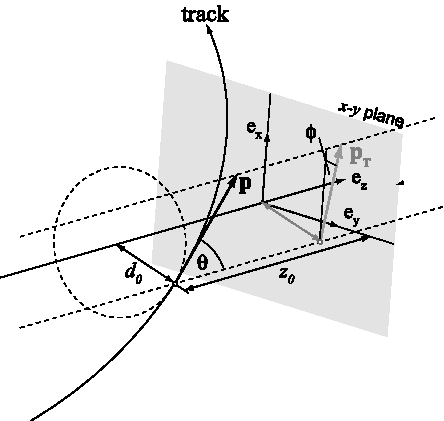
\includegraphics[width=0.6\textwidth]{plots/atlas/trackcoordinates.pdf}
    \caption{Schematic of the track coordinates defined using the perigee of the track. Figure from \cite{Atlas:trackcoords}\label{fig:trackcoords}.}
\end{figure}

Track reconstruction is partitioned into a primary tracking chain of algorithms followed by a back-tracking chain. %In the primary tracking, the track reconstruction is initiated by ``track seed'' formation in the pixel or SCT and in final step of, information from the TRT is used. The back-tracking chain is designed to resolve track ambiguities and is relevant primarily for the reconstruction of electron tracks from photon conversion. 
The primary tracking chain starts with track seed formation. Track seeds consist of a triplet of space-points (SP) in the pixel or SCT layers, which are consistent with originating from a charged particle track. Next, for each seed, a set of detector modules in the path of the track are identified. The seeds are extended using SCT and pixel clusters contained within those modules using a Combinatorial Kalman Filter \cite{Atlas:kalman}. This results in a set of potentially overlapping track candidates. Fake tracks also are reconstructed, which are incorrect combinations of unrelated pixel and SCT clusters \cite{Atlas:trackingsoftwaretut}.

A dedicated ambiguity resolution step is performed to reduce contributions from fake tracks. In this step, a score is given to each track candidate based on a number of criteria, and lower quality candidates are rejected if there are a large number of shared hits with higher quality tracks. After the ambiguity resolution, a global $\chi^2$ fit is performed to obtain the final track parameters. Finally, if an extension of the track into the TRT is possible, tracks are extended, and a re-fit of the entire track is performed. For electron and converted photon tracks, there is an additional refitting procedure using a ``Gaussian-sum Filter'' (GSF) which is a generalisation of the Kalman filter. The GSF method takes into account non-linear effects related to bremsstrahlung \cite{Atlas:egam_reco_gsf}.  
%\begin{figure}[H]
%    \centering
%    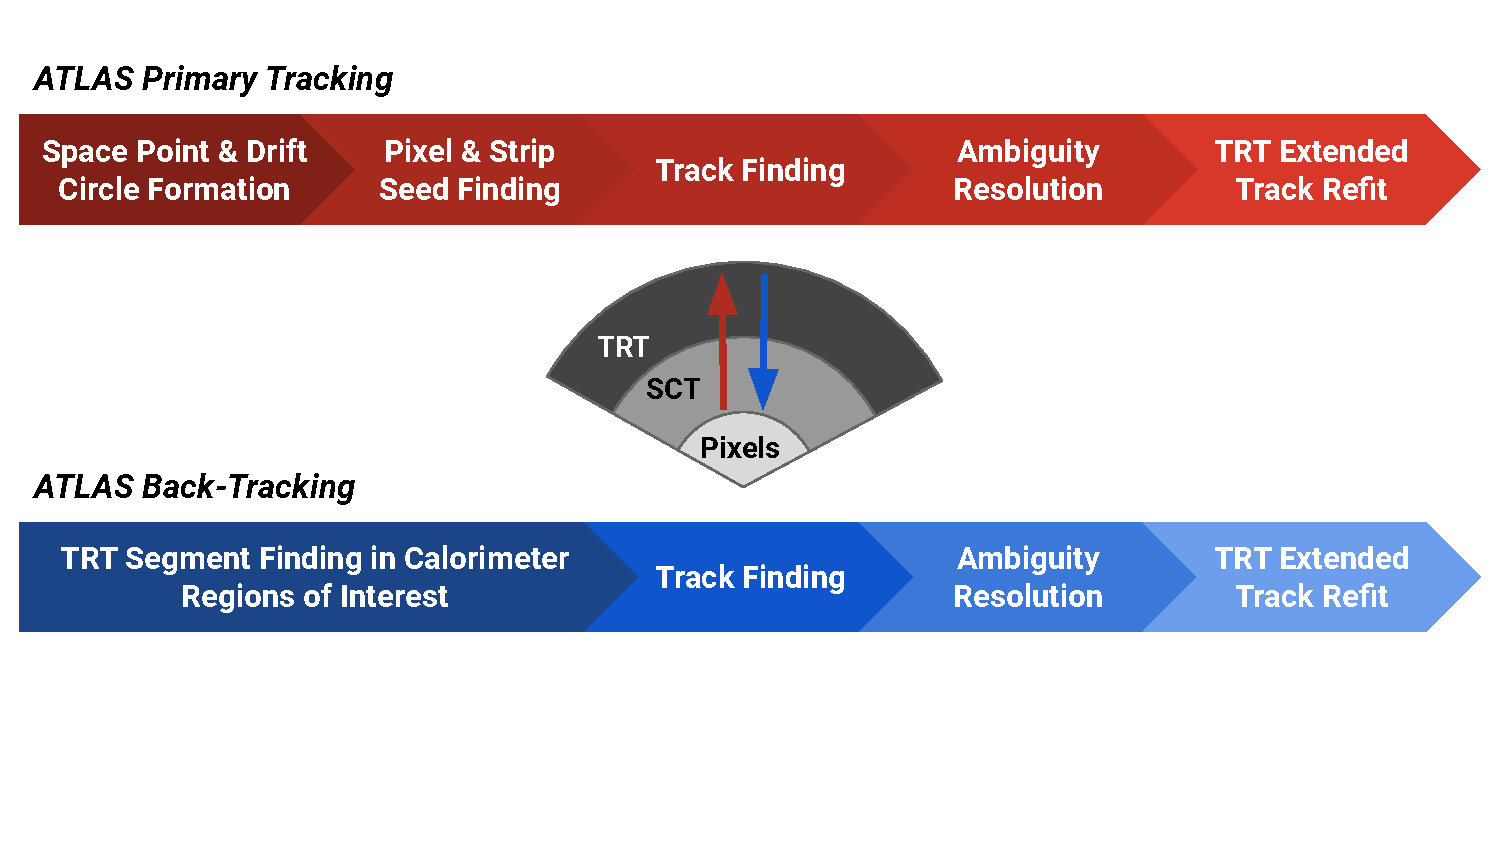
\includegraphics[width=0.8\linewidth]{plots/atlas/outin_tracking.pdf}
%    \caption{Illustration of primary and secondary tracking chains using in ATLAS track reconstruction. From \cite{Atlas:trackreco_run3}.\label{fig:outin_tracking}}%consider removing?
%\end{figure}

To increase the acceptance of the tracking to particles produced away from the beamline, such as electrons originating from photon conversions, tracks are reconstructed from the outside-in (seeded by the TRT) using detector hits not already associated with tracks from the primary pass. To avoid large contributions from falsely reconstructed tracks backtracking is only performed in regions seeded by energy deposits (\et > 6 GeV) in the EM calorimeter \cite{Atlas:trackreco_run3}.

With the mean number of interactions per bunch-crossing being $\langle\mu\rangle=33.7$ for Run-2 \cite{Atlas:mu}, precisely identifying the specific $pp$ interactions, called primary vertices \footnote{``Primary'' refers to $pp$ interactions. Secondary vertices are defined as the spatial locations of hadronic interactions from primary ($pp$) collision products. From here on, the term ``vertex'' will be used to refer to a primary vertex \cite{ATLAS:sv}.}, is an important task. An iterative vertex finding algorithm, which takes all tracks as input parameters, is used for vertex reconstruction. %The first vertex is reconstructed using all tracks, and in each subsequent iteration, the vertex position is refined. After the last iteration, tracks that are incompatible with the vertex are returned to the pool of unused tracks, which are then considered as inputs for a new vertex. The end result is a set of three-dimensional vertex positions and their covariance matrices.
The hard-scatter vertex is usually identified amongst many pileup vertices as the vertex which has the largest $\sum\pt^2$ of contributing tracks. The assumption here is that the charged particles produced in the hard-scatter interaction have a harder \pt spectrum than those produced in pile-up interactions \cite{Atlas:trackreco_run3, Atlas:pvreco}.

\subsubsection{Electrons and Photons}\label{sec:egamma}
Electrons and photons can be identified by the presence of a shower in the EM calorimeter. The showers of electrons and photons are almost indistinguishable, since electrons emit photons through bremsstrahlung, and photons produce electron-positron pairs. However, since the ID only responds to charged particles, photons and electrons can be distinguished through the presence or absence of a track.

Electrons are experimentally defined as objects consisting of a cluster built from energy deposits in the calorimeters and one or more matched tracks. Converted photons are defined as calorimeter clusters matched to a photon conversion vertex. Unconverted photons are defined as clusters without either a matched conversion vertices or an electron track. 

Electron and photon reconstruction starts with a topological cluster (topo-cluster) formation algorithm. Topo-clusters are topologically connected collections of EM and hadronic calorimeter cells, calibrated at the EM scale\footnote{The EM Scale is derived using electron test beams and is defined as the mean calorimeter response measured as the ratio of deposited charge to test-beam energy. The EM scale therefore corrects the measured calorimeter signal to the correct energy for EM showers.}. The algorithm starts with the formation of seed cells, which are required to have a cell energy of at least four times the expected cell noise. Neighbouring cells are then connected if the cell energies are at least twice the expected cell noise. These clusters of cells then go on to become the seed cells for the next iteration, and proto-clusters are merged if they share cells. In the final splitting step, proto-clusters are split into separate clusters if they contain two or more local maxima ($E_{\text{cell}}>500\MeV$ and $\geq4$ neighbours with a smaller signal).

Topo-clusters contain both EM and hadronic calorimeter cells, however, only the energy measured from cells in the EM calorimeter are used for photon and electron reconstruction. Energy measurements in the hadronic calorimeter are still important, however, since they are used to quantify the fraction of the EM calorimeter energy to the total cluster energy, $\mathit{f}_{\text{EM}}$. Topo-clusters with $\mathit{f}_{\text{EM}} > 0.5$ are called EM topo-clusters. Each topo-cluster is interpreted as a massless pseudo-particle, and the energy and momentum components are calculated from the cluster energy at the EM scale and the angular coordinates of the cluster. The reason for defining clusters as massless is because there is no physically meaningful mass without a corresponding particle hypothesis for the origin of the signal \cite{Atlas:topoclusters}. The reconstruction is finalised with the matching of tracks and conversion vertices to clusters using a $\Delta R$ criteria \cite{Atlas:egam_reco}.
%\newline
%A track is considered matched to a topo-cluster if there is small $\Delta\eta$, and a small $\Delta\phi$ separation between the track and the cluster. There is a similar requirement to match conversion vertices to topo-clusters. After matching tracks to topo-clusters, electron and photon ``superclusters'' are seeded from topo-clusters. Superclusters are dynamic, variable sized clusters of calorimeter cells. To build the superclusters, EM topo-clusters are sorted in descending \et. For a cluster to become an electron seed, it must have $\et>1\GeV$, and it must be matched to a track with at least four hits in the Pixel + SCT detectors. For photons, the seed energy threshold is $\et>1.5\GeV$. To capture EM showers originating from the same initial electron or photon, ``satellite'' clusters are identified using an $\eta-\phi$ window of size $0.075\times0.125$ around the centre of the seed cluster. For electrons, a secondary cluster is also considered a satellite if it shares the same best-matched track with the seed, and the secondary cluster is within a larger $\eta-\phi$ window of size $0.125\times0.300$. For converted photons, secondary clusters are considered satellites if they share the same conversion vertex, or if the secondary cluster is matched to a track that belongs to the conversion vertex. The seed clusters and their associated satellites are called superclusters. After this, tracks and conversion vertices are matched to superclusters, and there is an additional ambiguity resolution step to resolve cases where a given seed produces both an electron and a photon. The ambiguity is either resolved or these objects are explicitly marked as ambiguous. The reason for using superclusters as opposed to fixed-sized clusters (fixed-sized clusters were used for early run-2 analyses) is the improved energy resolution, especially in the forward detector regions for electrons and converted photons. In these cases, the improvements can be as large as 40\%.\cite{Atlas:egam_reco} 
%\newline

After reconstruction, electrons and photons are calibrated to account for energy losses in material upstream of the calorimeter, energy deposited outside of the clusters, and energy losses beyond the EM calorimeter. The electron/photon energy scale\footnote{The energy scale is numerical factor that corrects the measured energy to that of simulated truth particles as a function of $\eta$ and \et or \pt.} is determined in a calibration chain, where the response of electrons and photons is derived from simulated samples \cite{Atlas:egamcal_run2,Atlas:egamcal_run1}. After the simulation-based correction is applied, additional corrections are derived using data to account for response variations not included in simulation, and non-linear behaviour of the electronics \cite{Atlas:egamcal_fullrun2}. Finally, a residual energy scale correction factor, called the in-situ calibration, is applied to data so that it agrees with the expectation from simulation. Additionally, a correction factor is applied to simulation so that the energy resolution agrees between data and simulation. These factor are derived using the $m_{ee}$ invariant mass distribution in $Z\rightarrow ee$ events, where a $\chi^2$ minimisation simultaneously solves for the energy scale and resolution parameters in bins of $\eta$. For photons, there is an additional correction to account for the mis-modelling of out-of-cluster leakage. This is only derived for photons since the mis-modelling is found to be lower than 0.1\% for electrons. The photon energy scale calibration is cross-checked using $Z\rightarrow ee\gamma$ decays, and the electron energy scale is validated with $J/\psi(c\bar{c})\rightarrow ee$ events in data \cite{Atlas:egamcal_run1,Atlas:egamcal_fullrun2}. The calibration chain used for correcting the full 140\infb Run-2 dataset is shown as a schematic in Figure \ref{fig:atlas_egamcali}.

\begin{figure}[t]
    \centering
    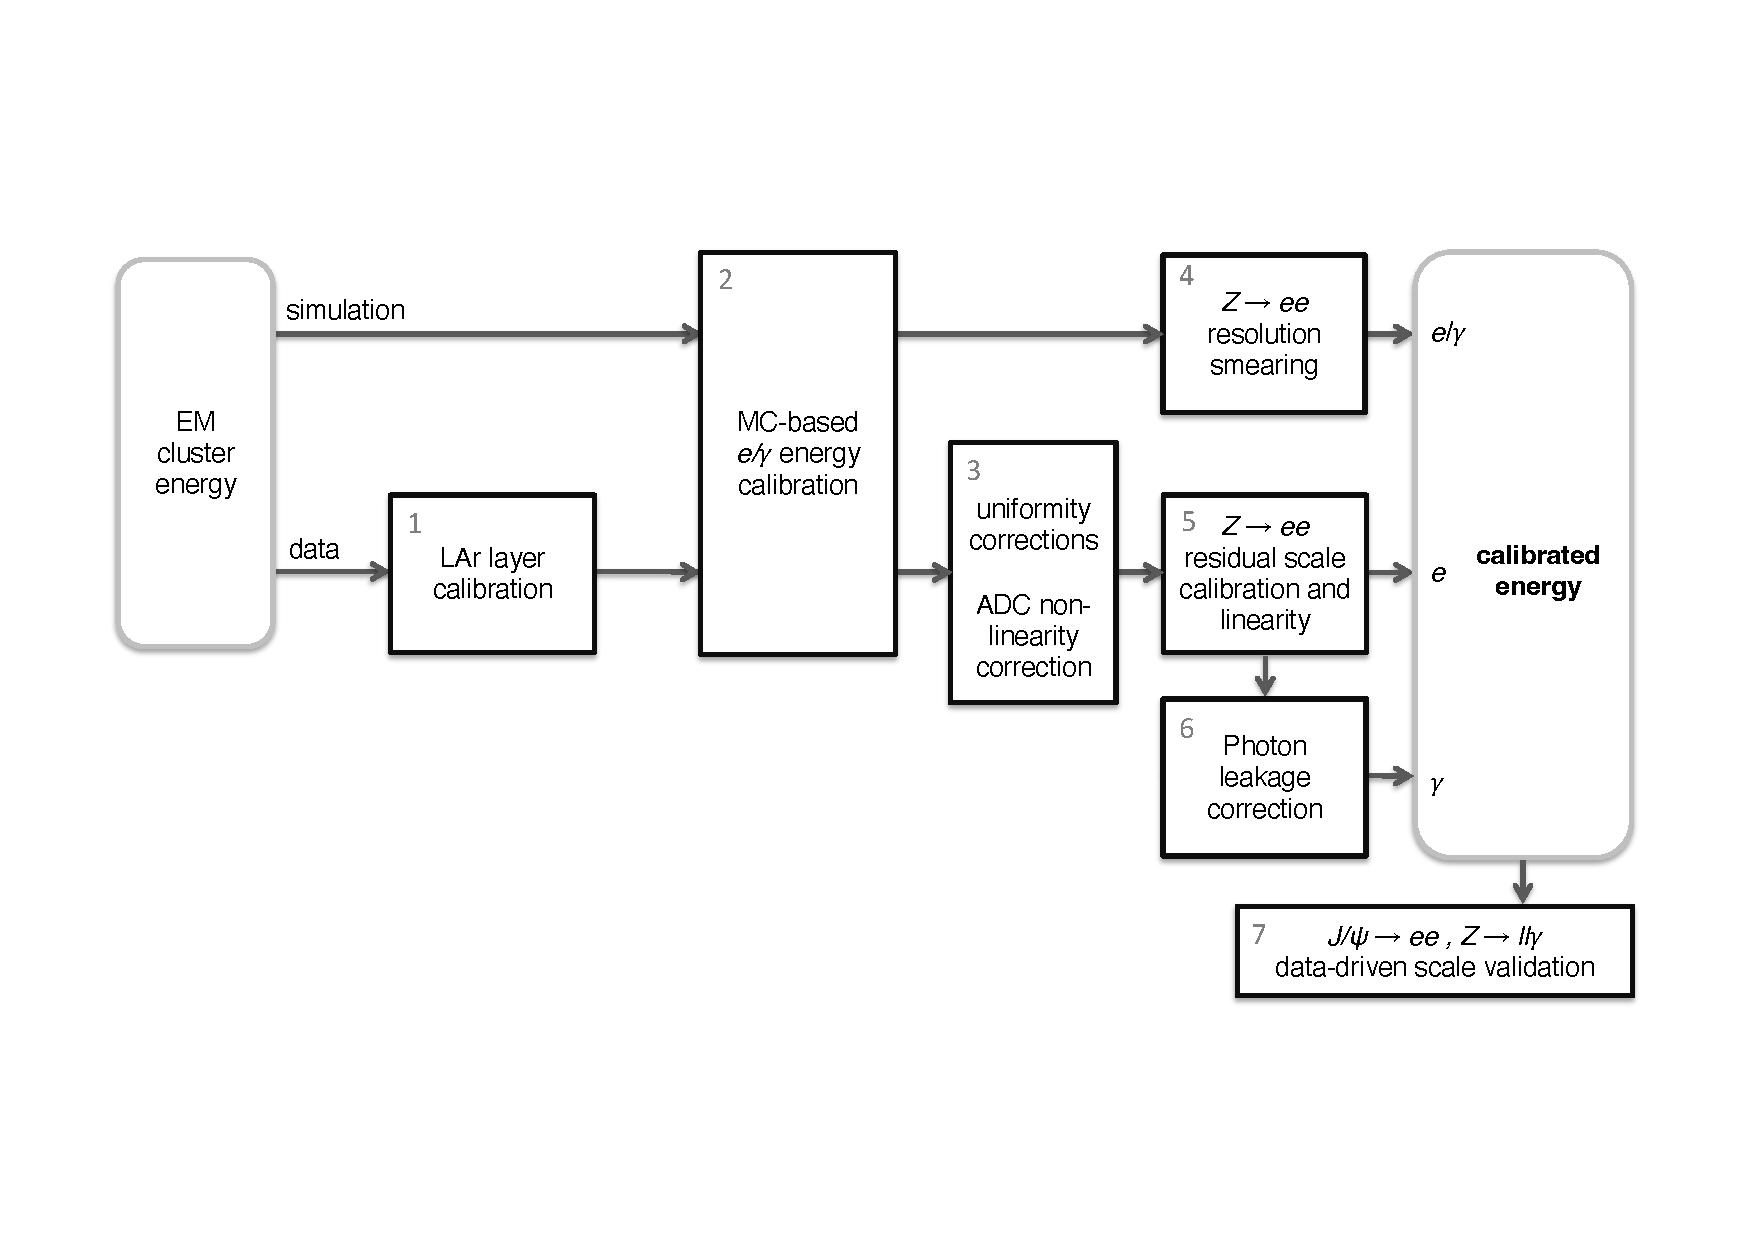
\includegraphics[width=\textwidth]{plots/atlas/egammacali.pdf}
    \caption{The $e/\gamma$ calibration chain used to correct the full Run-2 ATLAS dataset. Figure from \cite{Atlas:egamcal_fullrun2}.\label{fig:atlas_egamcali}}
\end{figure}
Electrons and photons can be mimicked by other objects, particularly jets, converted photons and heavy-flavour hadron decays. It is actually very rare for a jet to be collimated in addition to being almost entirely contained in the EM calorimeter \cite{Atlas:egamcal_run2}. After reconstruction and calibration, identification algorithms based on shower shape variables are calculated to separate prompt\footnote{The definition of a prompt lepton are those not from hadron decays. Prompt photons are those not from hadron or $\tau$ lepton decays \cite{Atlas:truthdefs}.} electron/photons from jets. These variables quantify the degree to which the shower is collimated (the lateral shower development), how deep the shower penetrates the calorimeters (the longitudinal shower development), and in the case of electrons, the spatial compatibility of the track with the cluster.

Prompt electrons entering the central region ($|\eta|<2.47$) of the detector are selected using a likelihood-based (LH) identification (ID) discriminant \cite{Atlas:egam_reco}. By cutting on values of this discriminant, a given electron candidate can pass or fail \textit{Tight}, \textit{Medium}, \textit{Loose}, or \textit{VeryLoose} ID criteria. An electron satisfying a tighter working point has lower reconstruction efficiency but is more likely to correspond to a prompt electron. The likelihood discriminant is determined from signal and background probability density functions (pdf\footnote{pdf refers to probability density function, and PDF (capitalised) refers to parton distribution function.}). The signal pdfs are derived from $Z\rightarrow ee$ and $J/\psi\rightarrow ee$ events with a strict requirement on one of the reconstructed electrons and a very loose requirement on the other electron. The background pdfs are derived in a dijet enriched, prompt electron deficient fiducial region.

For photon identification within the region of $|\eta|<2.37, 1.37 < |\eta| < 1.52$ excluded, a cut-based, selection is implemented. Photon ID criteria are designed to select prompt, isolated photons, and reject backgrounds from jets. Eleven shower shape variables are used to define \textit{Tight}, \textit{Medium}, and \textit{Loose} (the latter two are used in the trigger) working points. Additionally, there are multiple photon ID working points for variations of the \textit{Tight} selection, where a number of shower-shape variable cuts have either been removed, or relaxed. These are called \textit{LoosePrime2-5}. These working points are useful for estimating systematic uncertainties on non-prompt photon estimates \cite{Atlas:egam_reco,Atlas:egamcal_run2}. 

The degree to which reconstructed electrons or photons are surrounded by other particles can be quantified using calorimeter or track based isolation variables. The calorimeter-based isolation energy ($E_{\text{T}}^{\text{coneXX}}$) is calculated by summing up the energy of topo-clusters whose barycentre\footnote{The barycentre of a topo-cluster is the average position of the cluster, weighted by energy deposits.} falls within a fixed-size cone of size $\Delta R$ of the EM particle cluster barycentre ($E_{\text{T,raw}}^{\text{isolXX}}$), and subtracting the energy contributed by the electron or photon which is taken to be a fixed $\Delta\eta\times\Delta\phi=5\times7$ cluster around the barycentre of the EM particle cluster ($E_{\text{T,core}}$). An additional leakage correction ($E_{\text{T,leakage}}$) is required to account for the fact that not all of the EM particle energy is subtracted. Finally, there is a correction to account for pileup and underlying-event\footnote{The underlying event (UE) is usually defined as all particles from a single particle collision except those from the process of interest. The UE is not equivalent to minimum bias events, but they are related \cite{Atlas:ue}.} ($E_{\text{T,pile-up}}$). The full calorimeter-based isolation energy is expressed as:
\begin{equation}
    E_{\text{T}}^{\text{coneXX}}=E_{\text{T,raw}}^{\text{isolXX}}-E_{\text{T,core}}-E_{\text{T,leakage}}(E_{\text{T}},\eta,\Delta R)-E_{\text{T,pile-up}}(\eta,\Delta R),
\end{equation}
where XX refers to the size of the cone, $\Delta R=\text{XX}/100$. The track isolation variable ($p_{\text{T}}^{\text{coneXX}}$) is calculated by summing the \pt of tracks within a cone centered around the electron track or photon cluster direction, whilst excluding the tracks matched to the electron or converted photon. Track-based isolation has better resolution and lower pile-up dependence and provides a superior \pt resolution. However, calorimeter-based isolation includes neutral particles and particles below the ID track \pt threshold. Hence, both variables provide complimentary information, and the combination of selections on both variables generally results in improved performance over cutting on one variable \cite{Atlas:egam_reco}.

Electron isolation working points include the \textit{Gradient} working point which is defined such that the selection efficiency is $95\%$ at $\pt = 20\GeV$ and $99\%$ at $\pt = 60\GeV$, as well as \textit{Loose}, \textit{Tight}, and \textit{HighPtCaloOnly} which implement a cut on the calorimeter or track isolation variables as a function of \pt. The \textit{HighPtCaloOnly} working point gives the largest rejection of all the working points at high \pt, and only uses the calorimeter-based isolation variable. There are three photon isolation working points: \textit{Loose}, \textit{Tight}, and \textit{TightCaloOnly}. These all cut on the isolation variables as a function of \et, and the \textit{TightCaloOnly} working point only uses the calorimeter-based isolation variable. 

Differences between data and simulation can arise due to imperfect detector modelling (see Section \ref{sec:dataproc} for more details), mismodelling of the shower shape variables, as well as the modelling of complex objects such as the beamspot. The ratios of the data-to-MC efficiencies are referred to as ID or isolation efficiency scale factors, or just scale factors, and correct the MC simulations so that they closely resemble the data. Systematic variations in these scale factors are propagated through to the analysis-level objects \cite{Atlas:photonid_run2}.

%TODO: Define barycentre and the likelihood discriminant

%These variables capture things like ratios of energy deposited in a particular layer of the calorimeter relative to that deposited in another layer or relative to the total cluster energy, as well as lateral shower widths.
%Could mention improved energy resolution that superclusters provide (presumably over old sliding window algorithms?). Width quantified using inter-quartile-range, IQE.
%Discuss electron and photon energy calibration next. After the calibration, the shower shape variables and other discriminating variables are calculated for electron and photon ID.

\subsubsection{Muons\label{sec:muon}}
 
Muons can be reconstructed solely using the MS (stand-alone muons), or a combination of detector subsystems. Stand-alone muons are of use in the reconstruction of ID + MS combined muons and when operating in the forward region $2.5 < |\eta| < 2.7$, which is not covered by the ID. Stand-alone muon reconstruction starts with track reconstruction in the MS, where preliminary track candidates are formed through the identification of short straight-line track segments from hits in individual MS stations. The tracks are then built using all MS subdetectors, taking into account detector-misalignment, particle-detector interactions, outlier hits, track overlaps, and calorimeter energy losses. Track candidates are finalised after being extrapolated to the IP \cite{Atlas:muonreco}.%precision three-dimensional track coordinates are constructed using information from all of the MS subdetectors. Muon trajectories are built with a global $\chi^2$ fit which takes detector misalignment and particle-detector interactions into account. In the next step, these trajectories have outlier hits removed, and hits compatible with the trajectory which were not originally assigned are added. The tracks are then refit with this updated information. In an ambiguity resolution step lower quality tracks are removed if they have a large overlap with high quality tracks. The final tracks are then refit with a loose IP constraint, taking energy losses in the calorimeters into account, and the tracks are extrapolated to the beam line.

In most cases, it is advantageous to combine the signals from the MS with other detector subsystems. Since muons are the only standard model particle that leave signatures in the MS, usually the combination of ID and MS information is sufficient. However, in some special cases it is advantageous for the full detector information to be used. There are four classes of reconstructed muons where detector information beyond the MS is used:
\begin{enumerate}
    \item Combined muon (CB) tracks are formed from a successful combination of stand-alone MS muons and ID tracks.
    \item Inside-out combined (IO) muons are reconstructed with an algorithm that extrapolates ID tracks to the MS whilst using the ID track, the calorimeter energy losses, and the MS hits in a combined fit. IO muons have some performance improvements over CB muons as they do not rely on the independently reconstructed MS track. Most analyses only select for combined (either CB or IO) muons as the combination of two tracks results in the best possible precision.
    \item Segment Tagged (ST) muons are required to have a tight angular matching of an ID track to at least one reconstructed MS segment, and the muon parameters are taken solely from the ID track fit. ST muons are of use when there is no fully reconstructed MS track, but only segments in layers of the MS. This can be the case with low \pt muons.
    \item Calorimeter-tagged (CT) muons require an ID track which is extrapolated into the calorimeters. Energy deposits compatible with a minimum ionising particle are used to tag the ID track as a muon, and the muon parameters are taken directly from the ID fit. CT muons are only of use when there is no MS track, which is possible for cases where there are known holes in the MS. The signatures for these muons are easily caused by other particles and hence CT muons have low purity (one minus hadron misidentification rate).
\end{enumerate}
Muon identification working points (\textit{Loose}, \textit{Medium}, and \textit{Tight}) are defined to moderate the prompt muon purity and reconstruction efficiency trade-off. This is achieved through requirements on the number of hits in ID layers and MS stations, track properties, and ID-MS compatibility variables. Non-prompt muons can come about due to semileptonic decays of light hadrons as well as heavy-flavour hadron decays. Since light hadron decays result in lower-quality muons, the working points are optimised to reject muons from light-flavour hadrons. Non-prompt muons from heavy flavour decays result in higher quality muon tracks and can usually therefore be distinguished from prompt muons through the association with the primary vertex and the isolation of the ID tracks or calorimeter deposits. In addition to the standard working points, \textit{Low-}\pt and \textit{High-}\pt working points are optimised to select for low and high \pt muons.

The track and calorimeter-based isolation variables for muons are defined in a similar way to electrons and photons (Section \ref{sec:egamma}). \pt requirements on the calorimeter and track-based isolation variables as well as a requirement on the track \pt give an array of isolation working points. These are \textit{Loose} and \textit{Tight}, in addition to more specialised working points such as the \textit{particle-flow} working points which are optimised to reject muons from heavy-flavour hadrons, as well as a set of track-only working points \cite{Buckley:PCP,Atlas:muonreco}.

\subsubsection{Jets\label{sec:atlas:jets}}
%The vast majority of $pp$ collisions at the LHC result in the production of quarks and gluons of which the observable signatures are collimated streams of hadrons, \textit{jets}. A number of algorithms for the clustering of observed detector outputs into jet objects exist, of which the primary one for ATLAS jet reconstruction is the anti-$k_t$ algorithm (Section \ref{sec:theory:jet}) with a distance parameter $R=0.4$. Four-momentum vector \textit{input objects} form the inputs to the algorithm, which may be derived from various sources. These are either tracks, calorimeter deposits organised into topo-clusters, or a combination of track and calorimeter information. The most common anti-$k_t$ distance parameter is $R=0.4$ (small-R jets), however, jets reconstructed with $R=1.0$ (large-R jets) are used in cases where high \pt jets originate from the hadronic decays of massive particles like H/W/Z bosons and top quarks. Since the angular separation of their decay products scales as $1/\pt$, i.e. $\Delta R\approx\frac{2m}{\pt}$, they become collimated (highly Lorentz-boosted) \cite{Atlas:altinputsjetgrooming}. In these situations, these decay products can be reconstructed in a single large-R jet.
The vast majority of $pp$ collisions at the LHC result in the production of quarks and gluons of which the observable signatures are collimated streams of hadrons, \textit{jets}. A number of algorithms for the clustering of observed detector outputs into jet objects exist, where the primary one for ATLAS jet reconstruction is the anti-$k_t$ algorithm (Section \ref{sec:theory:jet}). The most common anti-$k_t$ distance parameter is $R=0.4$ (small-R jets), however, jets reconstructed with $R=1.0$ (large-R jets) are used in cases where high \pt jets originate from the hadronic decays of massive particles like H/W/Z bosons and top quarks. Since the angular separation of their decay products scales as $1/\pt$, i.e. $\Delta R\approx\frac{2m}{\pt}$, they become collimated (highly Lorentz-boosted) \cite{Atlas:altinputsjetgrooming}. In these situations, these decay products can be reconstructed in a single large-R jet.

The inputs to the anti-$k_t$ algorithm are four-momentum vectors called \textit{input objects}, which can be derived from various sources. These are either tracks, calorimeter deposits organised into topo-clusters, or a combination of track and calorimeter information. Jets reconstructed solely from tracks are referred to as \textit{track-jets}. The acceptance limitations of the ID ($|\eta|<2.5$), and the inability for the ID to measure neutral particles limits the usefulness of track-jets. For this reason, jets in most ATLAS analyses are reconstructed solely using calorimeter topo-clusters, or a combination of topo-clusters and tracks. 
%Put this a bit later: At the heart of PFlow algorithms is the ability to distinguish the calorimeter energy deposits of neutral particles from charged particles. 
%\footnote{Athena is the name of the ATLAS software framework that manages almost all ATLAS production workflows including event generation, simulation, reconstruction and derivation production. All the work in this thesis uses Athena release 21, which was the release for run-2 data taking. Release 22 was used in initial run-3 data taking and is used in newer analyses for the reprocessing of run-2 data} 
% First year report

The formation of topo-clusters for jet reconstruction is identical to the description given in Section \ref{sec:egamma}. Calorimeter jets reconstructed at the EM scale are called \textit{EMTopo jets}. Calorimeter jets can also be reconstructed at the \textit{Local hadronic Cell-Weighting} (LC) scale, where an additional calibration factor is applied to topo-clusters consistent with hadronic energy deposits. These jets are called \textit{LCTopo} jets. The LC weighting is derived from simulations of single pion events, and corrects for signal losses and calorimeter non-compensation.

%It worth pointing out that further work is required to combine LC weighting with PFlow algorithms. Therefore, only jets reconstructed solely from calorimeter deposits are currently calibrated with the additional LC weighting
In Run-1 and in early Run-2 analyses, jets were reconstructed solely using topo-clusters. However, using a combination of ID and calorimeter information is preferable for the reasons that:
\begin{itemize}
    \item The calorimeters provide measurements of both charged and neutral particles.
    \item The superior angular resolution of the ID means that tracks can be associated with vertices.
    \item The momentum resolution of the ID at low \et is superior to that of the calorimeters. 
    \item The energy resolution of the calorimeters at high \et is superior to that of the ID.
    \item The calorimeters cover the forward $2.5<|\eta|<4.9$ regions.
\end{itemize}

%\subsubsection{The PFlow algorithm}
%
Different algorithms are used for the complimentary use of both track and calorimeter information. These algorithms are classified under the umbrella term of \textit{particle-flow}, or PFlow, algorithms \cite{Atlas:PFlowOG}\footnote{In this thesis, the terms \textit{particle/PFlow jets} and \textit{\textbf{the} particle/PFlow algorithm} will be used to refer to the particle flow algorithm described in \cite{Atlas:PFlow}. However, particle flow is a broader concept which can also be used to describe other input object algorithms. These are the TCC and UFO algorithms, and are described further on in this chapter.}. The PFlow algorithm described in \cite{Atlas:PFlow} was developed at ATLAS to combine tracking and calorimetric information for hadronic jet and soft activity\footnote{Soft activity is the additional hadronic recoil below the energy threshold used for jet reconstruction (this is important for missing transverse momentum reconstruction).} reconstruction. At the heart of this algorithm is the ability to distinguish charged from neutral particle deposits in the calorimeters and furthermore to subtract the energy deposited by charged particles from the topo-clusters and to replace them with the momenta of tracks matched to the topo-clusters. The output of the algorithm is a list of tracks, a list of unmodified topo-clusters, and a list of modified topo-clusters. These outputs are often referred to as a Particle Flow Objects (PFOs). The pion mass is assumed, since pions dominate the charged component of the jet, and to take up an average of approximately two-thirds of the visible jet energy \cite{Atlas:PFlow,Atlas:jetconstituent1,Atlas:jetconstituent2}. %Next, read through page 9-10 of pflow algorithm, decide which parts of that to add, maybe add the flow chart. Decide on which bits to elaborate on further. Maybe don't spend tooooo much time on PFlow stuff. Still need UFO, TCC, JER, JMR, calibration, Insitu. 

The steps of the PFlow algorithm are as follows:
\begin{enumerate}
    \item \textbf{Track selection}: Well-measured tracks are selected: 9 hits in the Pixel + SCT; no pixel holes; ID acceptance $|\eta|<2.5$; and $0.5\GeV<\pt<40\GeV$. The lower bound \pt threshold is chosen to allow for tracks from particles below the topo-cluster energy threshold. The upper bound selects against poorly isolated tracks. Tracks matched to electrons or muons with \textit{medium} ID are rejected since the algorithm is optimised for hadronic showers.
    \item \textbf{Matching tracks to topo-clusters}: For each track, an attempt is made to find a match with a single topo-cluster. In some cases tracks are determined to not have formed a topo-cluster. These tracks are retained in the algorithm output list of tracks and steps 3-6 are not performed.
    \item \textbf{Expected deposited particle energy}: The mean deposited energy of a track of measured momentum $p^{\text{trk}}$, denoted $\langle E_{\text{dep}}\rangle$, is determined using single-pion samples without pileup. Additionally, the spread in the expected single-pion energy deposition ($\sigma(E_{\text{dep}})$) is determined. These are important quantities for steps 4-6 of the algorithm. 
    \item \textbf{Split-shower recovery}: For each track/topo-cluster system, a discriminant $S(E^{\text{clus}})\equiv\frac{E^{\text{clus}}-\langle E_{\text{dep}}\rangle}{\sigma(E_{\text{dep}})}$, where $E^{\text{clus}}$ is the energy of the topo-cluster, is calculated to distinguish between cases where the particle energy is entirely deposited in a single topological cluster, and cases where the energy is split across multiple topo-clusters. This is actually very common, especially where the shower is split across two topo-clusters. A value of $E^{\text{clus}}>-1$ indicates that more than 90\% of clusters have the large majority ($>90\%$) of the particle's true energy deposited in the topo-cluster. Hence a discriminant value of $-1$ is used in performing the split-cluster recovery. The algorithm extrapolates the track to the EM calorimeter and expands the set of matched clusters using a simple $\DeltaR=0.2$ criteria around the extrapolated track.
    \item \textbf{Cell-by-cell subtraction}: It is possible that particles unrelated to the track (for example neutral particles) deposit their energy in close proximity to the clusters matched to the track. Hence simply removing every topo-cluster matched to a track would potentially remove energy deposits made these close-by particles. For this reason, the energy of the total set of topo-clusters is compared to $\langle E_{\text{dep}}\rangle$, and if it is less than $\langle E_{\text{dep}}\rangle$, the topo-clusters are removed. If total topo-cluster energy is larger than $\langle E_{\text{dep}}\rangle$, a cell-by-cell subtraction procedure is implemented to remove calorimeter cells around the extrapolated track.%$33.2\times\text{log}_{10}(40\GeV/{\pt^{\text{trk}}})$
    \item \textbf{Remnant removal}: If the cell-by-cell subtraction is implemented, it is likely that there will be some remaining energy from the cells that were not subtracted (if there are energy deposits from neutral particles, for example). A procedure is implemented to determine whether this energy is consistent with shower fluctuations, or whether the energy is consistent with close-proximity particle deposit(s). The remnant topo-clusters are removed if the former case, and retained in the latter.
\end{enumerate}
Figure \ref{fig:pflow} shows a flow chart of this PFlow algorithm.
\begin{figure}[t]
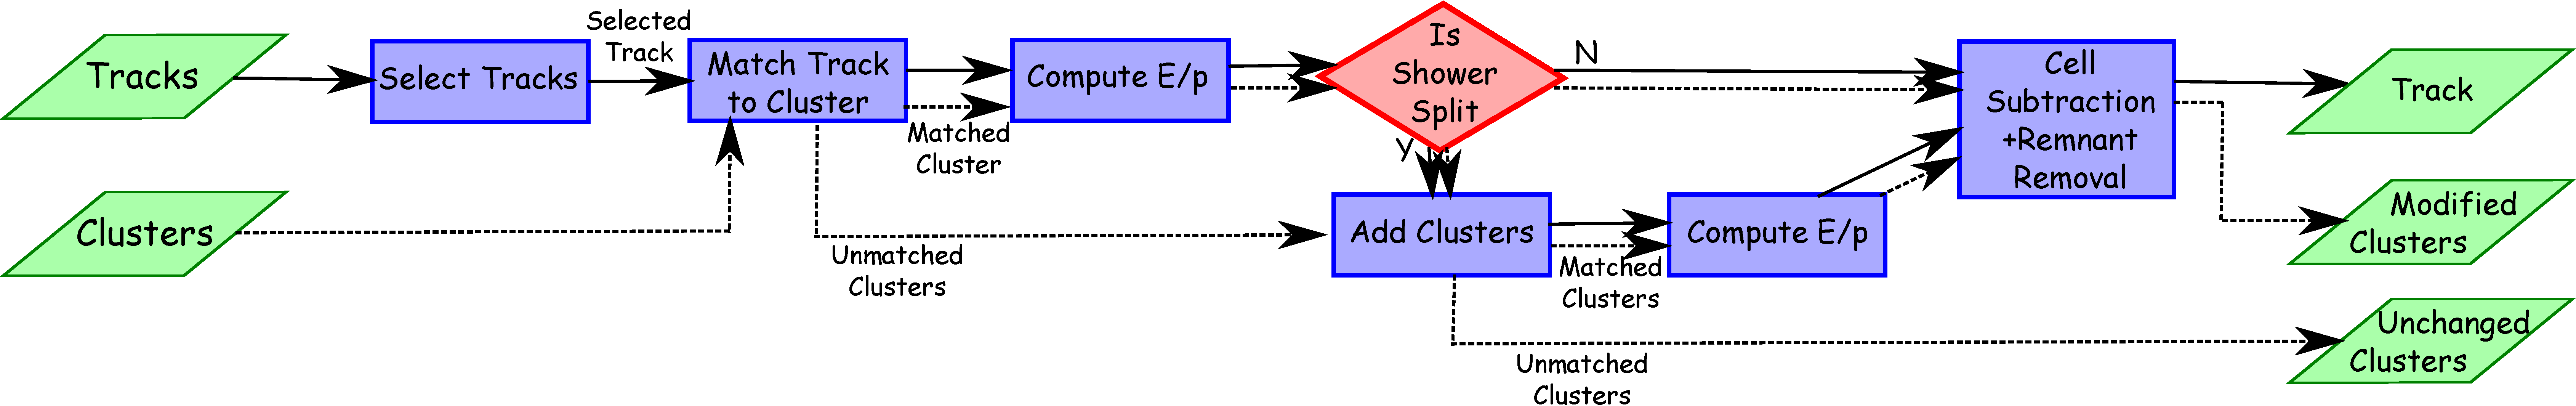
\includegraphics[width=\textwidth]{plots/atlas/pflow.pdf}
\caption{Flow chart showing the algorithm used in the construction of particle flow jet input objects. Figure from \cite{Atlas:PFlow}.\label{fig:pflow}}
\end{figure}

In the presence of pileup, where jets can arise from particles not produced in the primary hard scatter interaction, the performance benefits of PFlow jets can clearly be observed. This is shown in Figure \ref{fig:pflow_perf:a}, where the average number of pileup jets (referred to a ``fake jets'' in the figure) are compared between LCTopo jets and PFlow jets. The fake-rate is an order of magnitude lower for PFlow jets in the region of tracker acceptance, and there are no large deviations in performance outside of the tracker acceptance. Figure \ref{fig:pflow_perf:b} shows the efficiency of reconstructing a hard-scatter jet, and improvements to the hard-scatter jet reconstruction efficiency can be seen in the comparison of PFlow jets to LCTopo jets. 
\begin{figure}[t]
\centering
\begin{subfigure}[b]{0.46\textwidth}
    \centering
    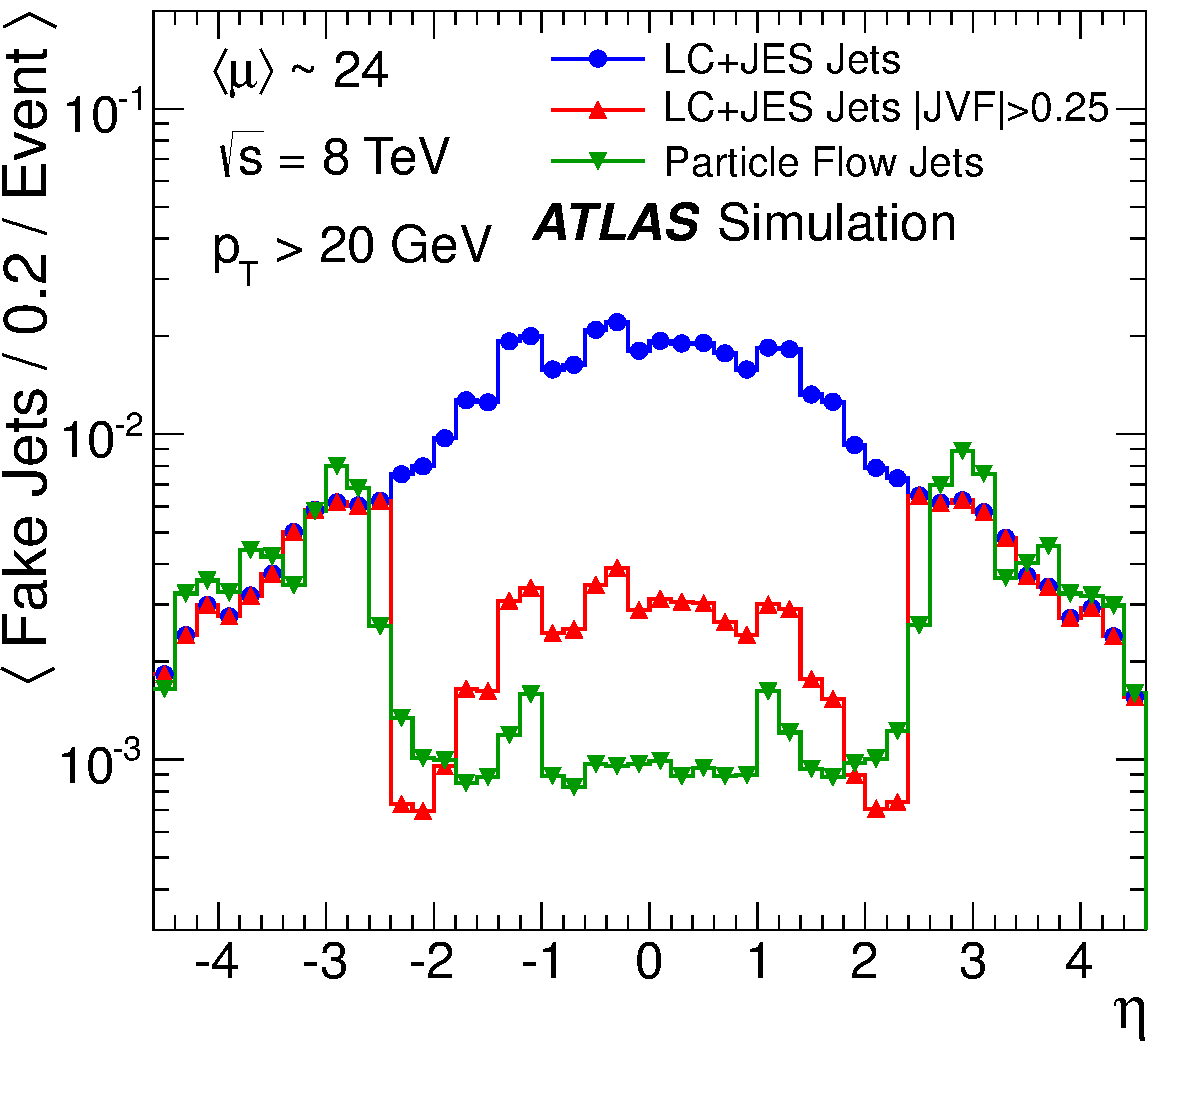
\includegraphics[width=\textwidth]{plots/atlas/pflow_performance_a.pdf}
    \caption{}
    \label{fig:pflow_perf:a}
\end{subfigure}
\hfill
\begin{subfigure}[b]{0.46\textwidth}
    \centering
    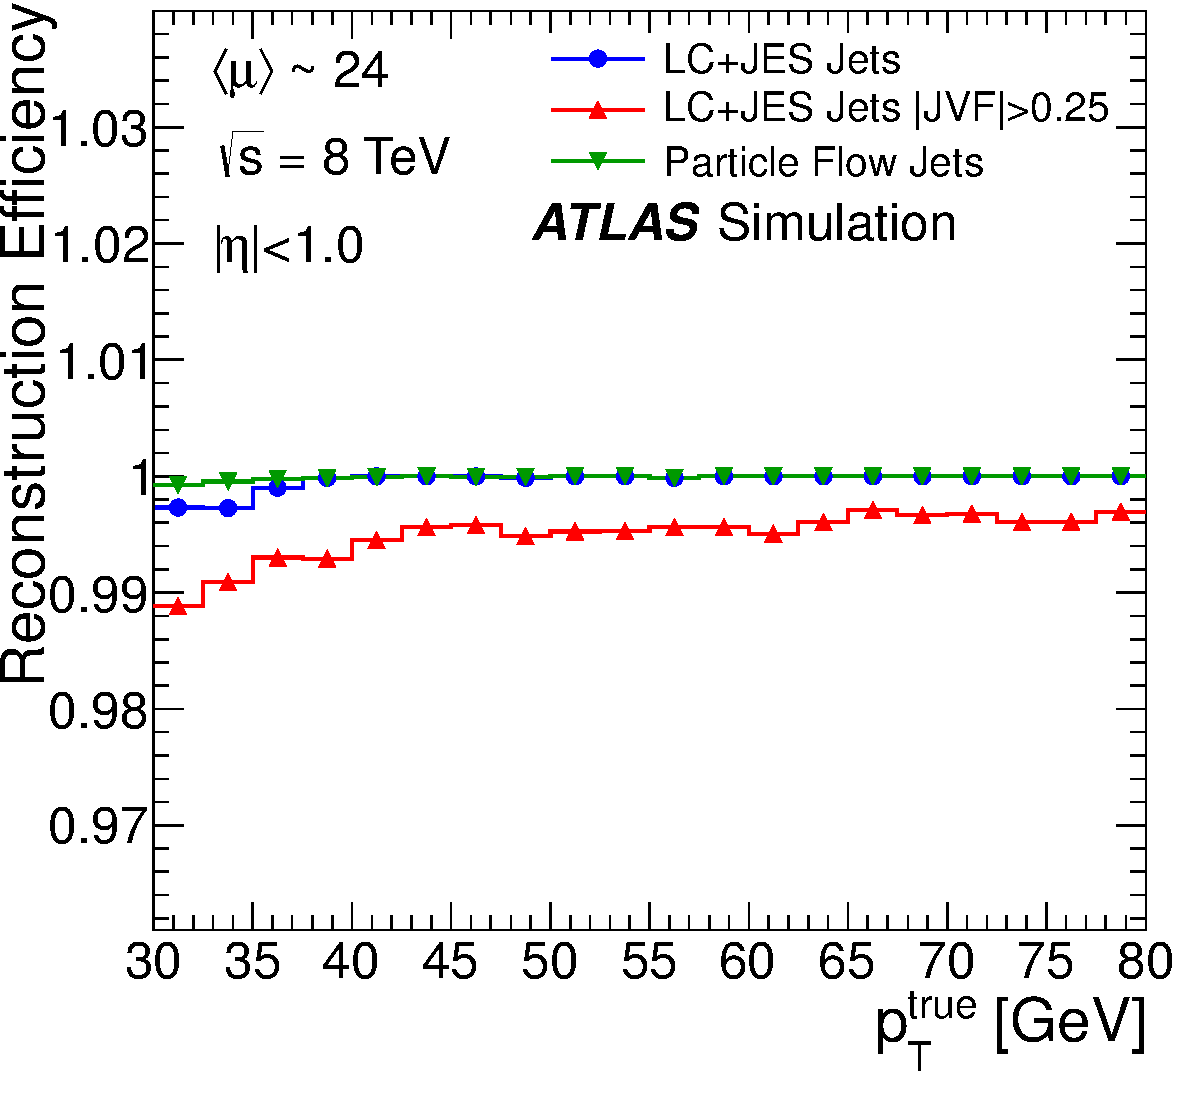
\includegraphics[width=\textwidth]{plots/atlas/pflow_performance_b.pdf}
    \caption{}
    \label{fig:pflow_perf:b}
\end{subfigure}
\caption{Performance improvements of PFlow jets over calorimeter jets. Figures from \cite{Atlas:PFlow}. with and without a jet vertex fraction (JVF) cut applied. JVF is the ratio of two scalar sums, where the numerator is the scalar sum of the \pt of tracks associated to the jets which are matched to the the hard-scatter vertex; and the denominator is the scalar sum of \pt of all tracks associated with the jet. \label{fig:pflow_perf}}
\end{figure}

In spite of the performance benefits shown in Figure \ref{fig:pflow_perf}, the algorithm does have some shortcomings, particularly at high \pt. Since the lateral shower width of a jet scales as 1/\pt, high \pt jets have a dense core. The presence of a dense core degrades the accuracy and efficiency of track reconstruction. Additionally, the angular resolution of the calorimeter limits the degree to which the cell subtraction step can be performed reliably in the presence of close proximity showers. It is because of these reasons, that tracks with $\pt > 40\GeV$ are excluded from the algorithm in the track selection step \cite{Atlas:PFlowOG}. 

%\subsubsection{The TCC algorithm}
Another PFlow algorithm called the Track-CaloCluster (TCC) algorithm \cite{Atlas:TCC} was developed at ATLAS for improved jet substructure reconstruction performance, and hence tagging performance in very high \pt jets. Since the energy resolution of the calorimeters is superior to that of the ID at high \pt, the TCC algorithm directly uses the energy information from topo-clusters and the angular information from tracks. The output of the TCC algorithm is a set of four-momenta (\pt,$\eta$,$\phi$,$m$), where $m$ is the invariant mass of the object\footnote{TCC objects are massless if $\leq 1$ topo-clusters are matched to the seed track, and have non-zero mass if multiple clusters are matched to the seed track}. The TCC algorithm works are follows:
\begin{itemize}
    \item All \textit{loose} tracks matched to primary vertices (including pileup) are matched to topo-clusters calibrated at the LC scale, and each track forms its own TCC object. In cases where one track matches one topo-cluster, the \pt of the TCC object is taken from the topo-cluster, and the $\eta$ and $\phi$ coordinates from the track.
    \item If multiple tracks match to multiple topo-clusters, the cluster \pt is split amongst the tracks, and the track angular coordinates are taken from the seed track.
    \item In cases where there is a topo-cluster (track) unmatched to a track (topo-cluster), the four-momentum of the TCC object is taken as that of the topo-cluster (track).
\end{itemize}
%\subsubsection{The UFO algorithm\label{sec:UFO}}
A particle flow algorithm called the Unified Flow Object (UFO) algorithm was designed as a solution to the problem that no single jet input object definition, be it PFlow, TCC or LC/EMTopo, is optimal for any given measure of performance. TCC jets, while having excellent tagging performance at high \pt, perform worse than LCTopo jets at low \pt. PFlow jets outperform LCTopo jets across the entire \pt range, particularly when it comes to pileup sensitivity. However, PFlow jets have significantly worse tagging performance than TCC jets at high \pt. 

The UFO algorithm combines the PFlow algorithm in \cite{Atlas:PFlow} and the TCC algorithm \cite{Atlas:TCC} in such a way as to optimise the performance across the kinematic range. In this algorithm, the $\pt^{\text{trk}}<40\GeV$ cut is replaced with a method to gradually switch from the PFlow cell subtraction to the TCC cell subtraction depending on $\pt^{\text{trk}}$, and on the measured calorimeter activity \cite{Atlas:PFlow2}. The switch is made if the energy $E^{\text{clus}}$ in a cone of size $\Delta R=0.15$ around the extrapolated particle satisfies:
\begin{equation}
    \frac{E^{\text{clus}}-\langle E_{\text{dep}}\rangle}{\sigma(E_{\text{dep}})}>33.2\times\text{log}_{10}(40\GeV/{\pt^{\text{trk}}}).
    \label{eq:denseenvironment}
\end{equation}
In this way, the PFlow cell subtraction algorithm is not implemented for cases where the track momentum is high, and in cases where the measured calorimeter activity is high, such as in very dense environments. Additionally, charged PFOs (tracks selected by PFlow algorithm) which are not matched to the hard-scatter vertex are removed in order to suppress contributions from pileup. This procedure is called ``Charged Hadron Subtraction'' (CHS). The neutral PFOs (modified or unmodified topo-clusters) have constituent-level (before jet building with anti-$k_t$) pileup mitigation algorithms applied that go by the names of ``Constituent Subtracton'' (CS) and SoftKiller (``SK''). These pileup mitigation algorithms are applied for both small-R and large-R jets. The full UFO algorithm is outlined in Figure \ref{fig:ufoalgorithm}. UFO jets will be the default for small-R and large-R jet definitions in Run-3 analyses.
\begin{figure}[t]
    \centering
    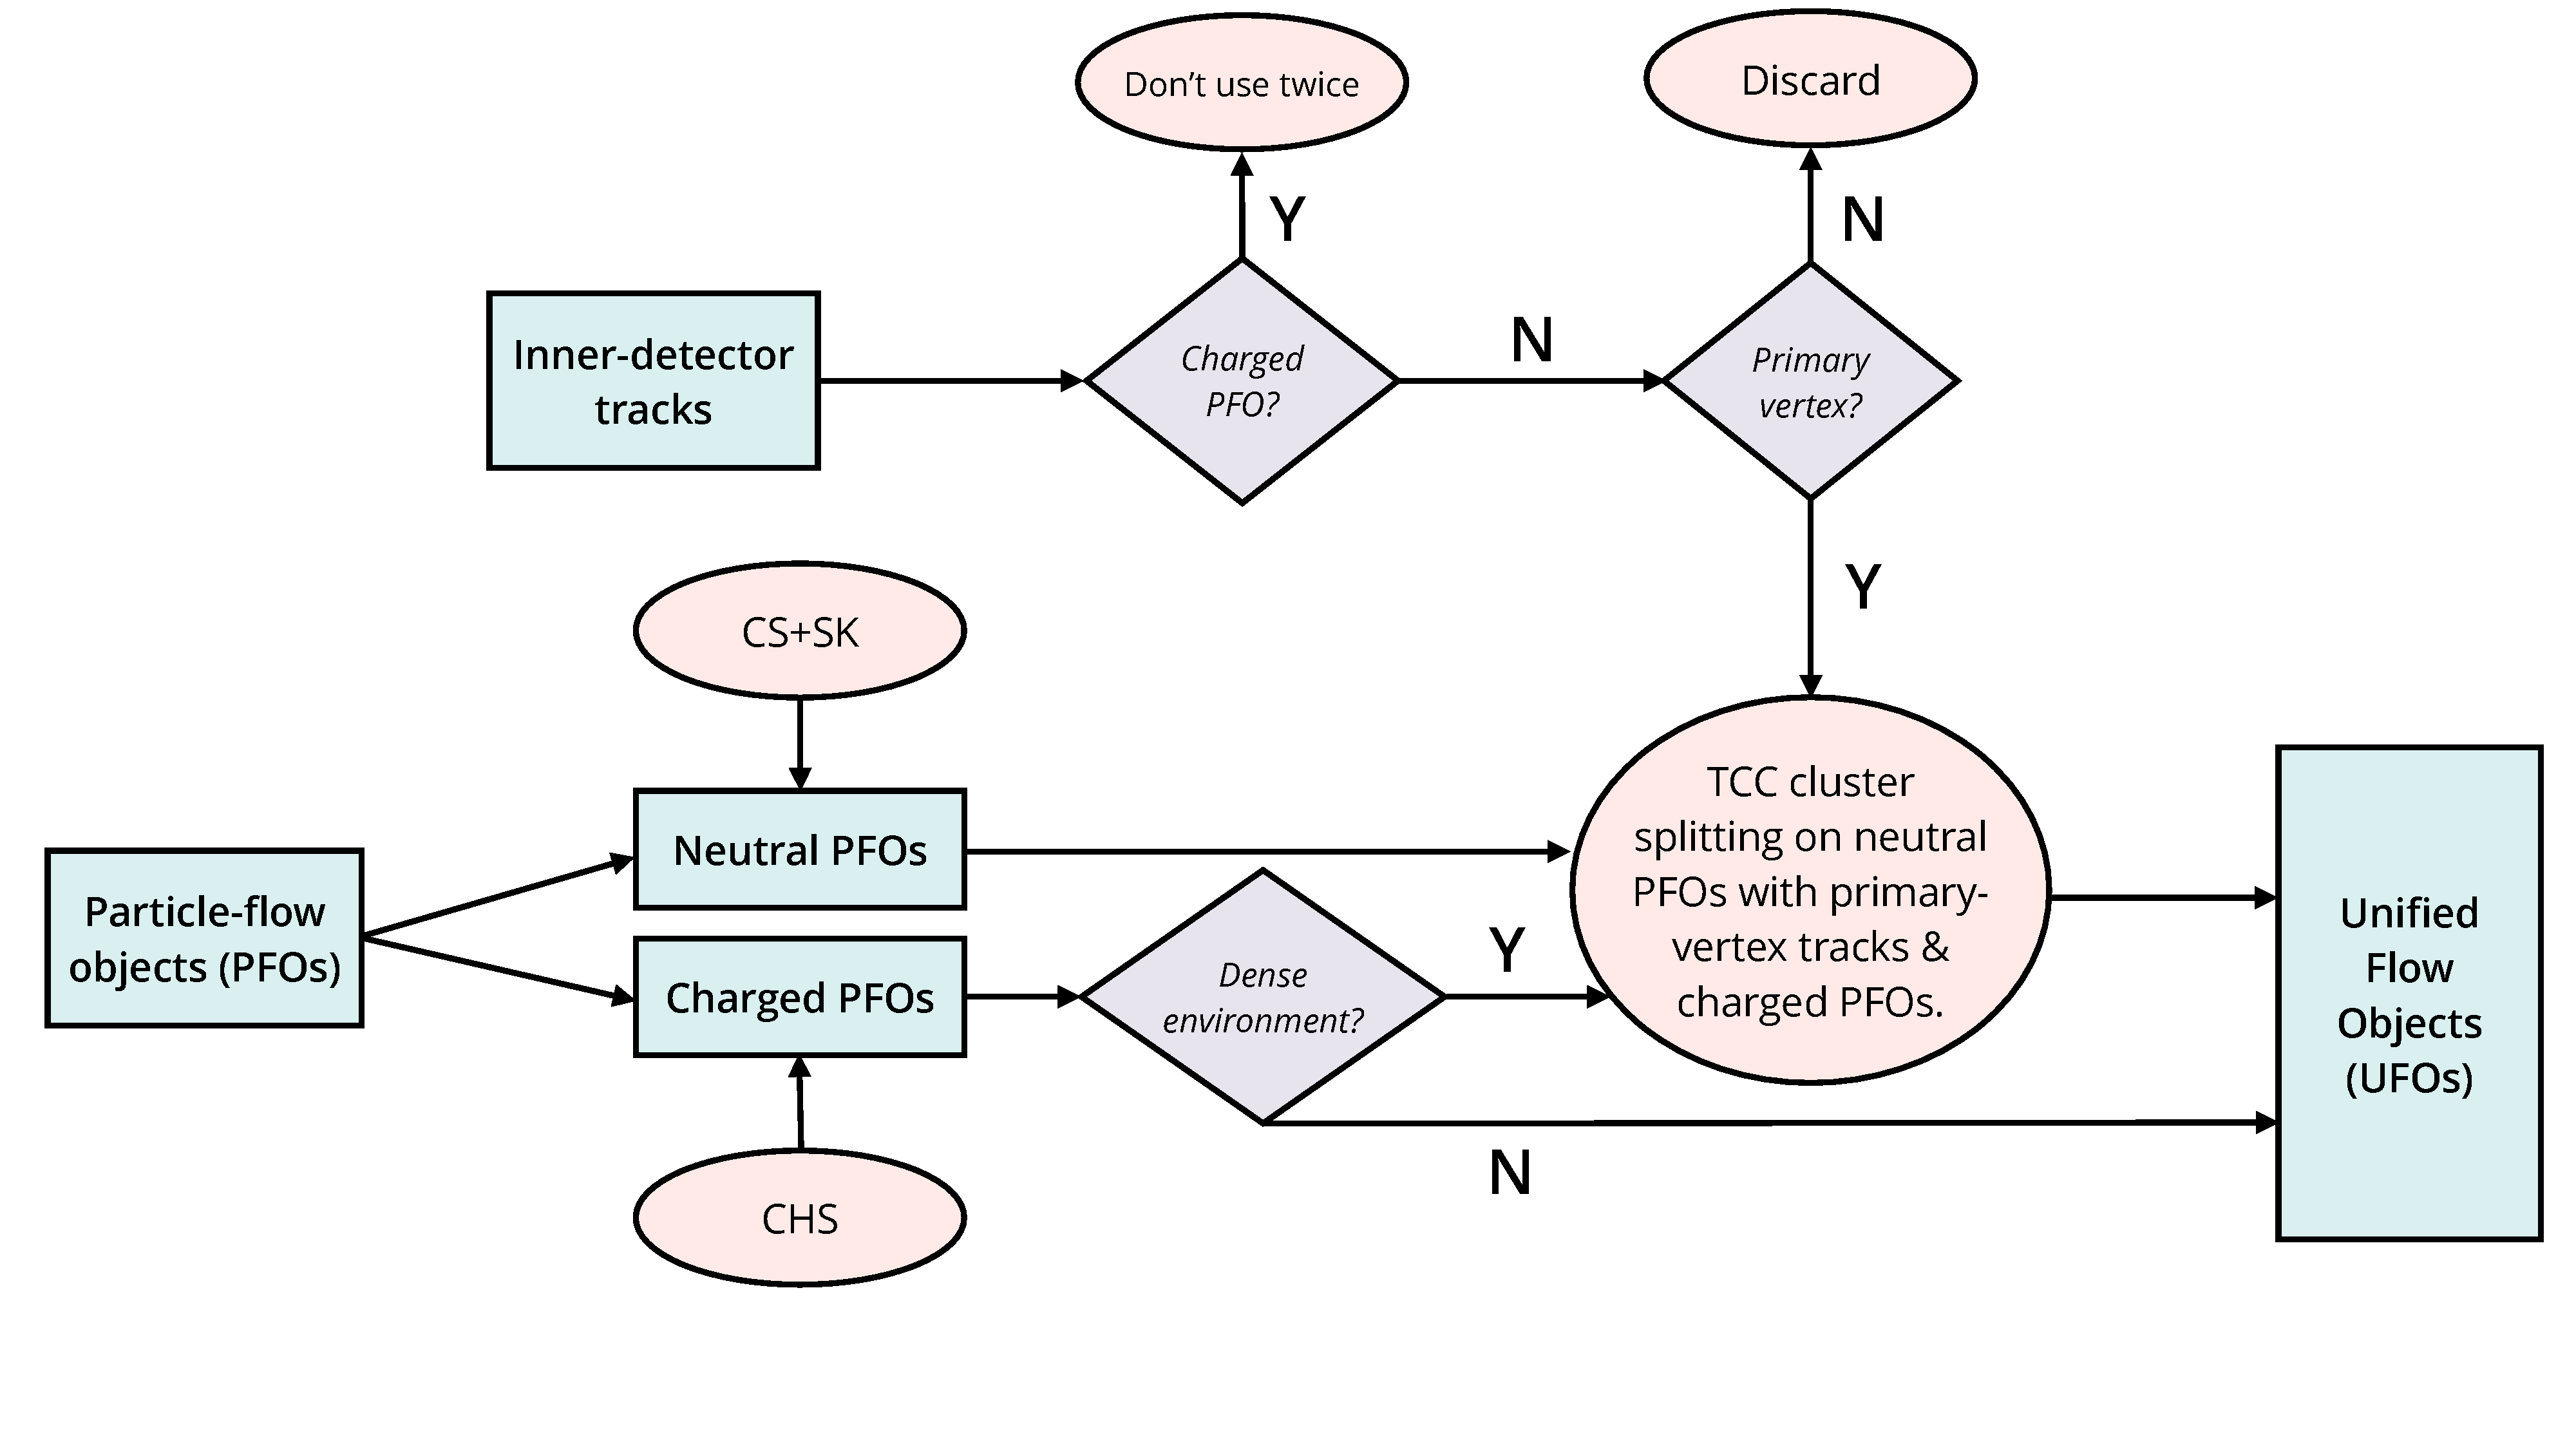
\includegraphics[width=\textwidth]{plots/atlas/ufoalgorithm.pdf}
    \caption{A flow chart outlining the construction of UFO jet input objects from PFOs and ID tracks. The ``dense environment'' decision is defined by equation \ref{eq:denseenvironment}, and results in the TCC algorithm being applied to track and topo-cluster combinations with high \pt tracks or very energy-dense calorimeter environments.\label{fig:ufoalgorithm}}
\end{figure}
%
%\subsubsection{Jet Energy Resolution (JER)}
%Precise knowledge of the JER is particular importance to precision SM measurements involving jets such as processes sensitive to VBS/VBF production, hadronic days of SM particles, in addition to BSM analyses involving jets. The JER is parametrised in form of equation \ref{eq:energyres}, where there is a contribution from a noise term, a stochastic term, and a constant term. The JER is often expressed in terms of \pt, as opposed to energy. Since the noise term is approximately independent of the energy deposited by the jet shower, the relative contribution from the noise term scales as $1/\pt$ and is thus more important at low \pt (below around 30\GeV). At around several hundred $\GeV$, the stochastic term dominates, which scales at $1/\sqrt{\pt}$. The constant term, which represents energy fluctuations that are a constant fraction of the jet \pt dominates above around 400\GeV. In order to measure the JER directly, a dijet momentum balance technique is used. Additionally, the noise term can be estimated directly through measurements of the fluctuations of the calorimeter energy deposits using pileup events from data samples with random unbiased triggers. The combined JER measurement is obtained using a technique similar to the combination of the different in situ JES measurements. The absolute JER uncertainty in the $\eta=0.2$ region as a function of \pt for 2017 data for calibrated PFlow and EMTopo jets is shown in figure \ref{fig:jer:a}. The absolute JER uncertainty with $\eta$ for 30\GeV jets is shown in figure \ref{fig:jer:b} \cite{Atlas:smallrcali}.
%
%\begin{figure}
%\centering
%\begin{subfigure}[b]{0.46\textwidth}
%    \centering
%    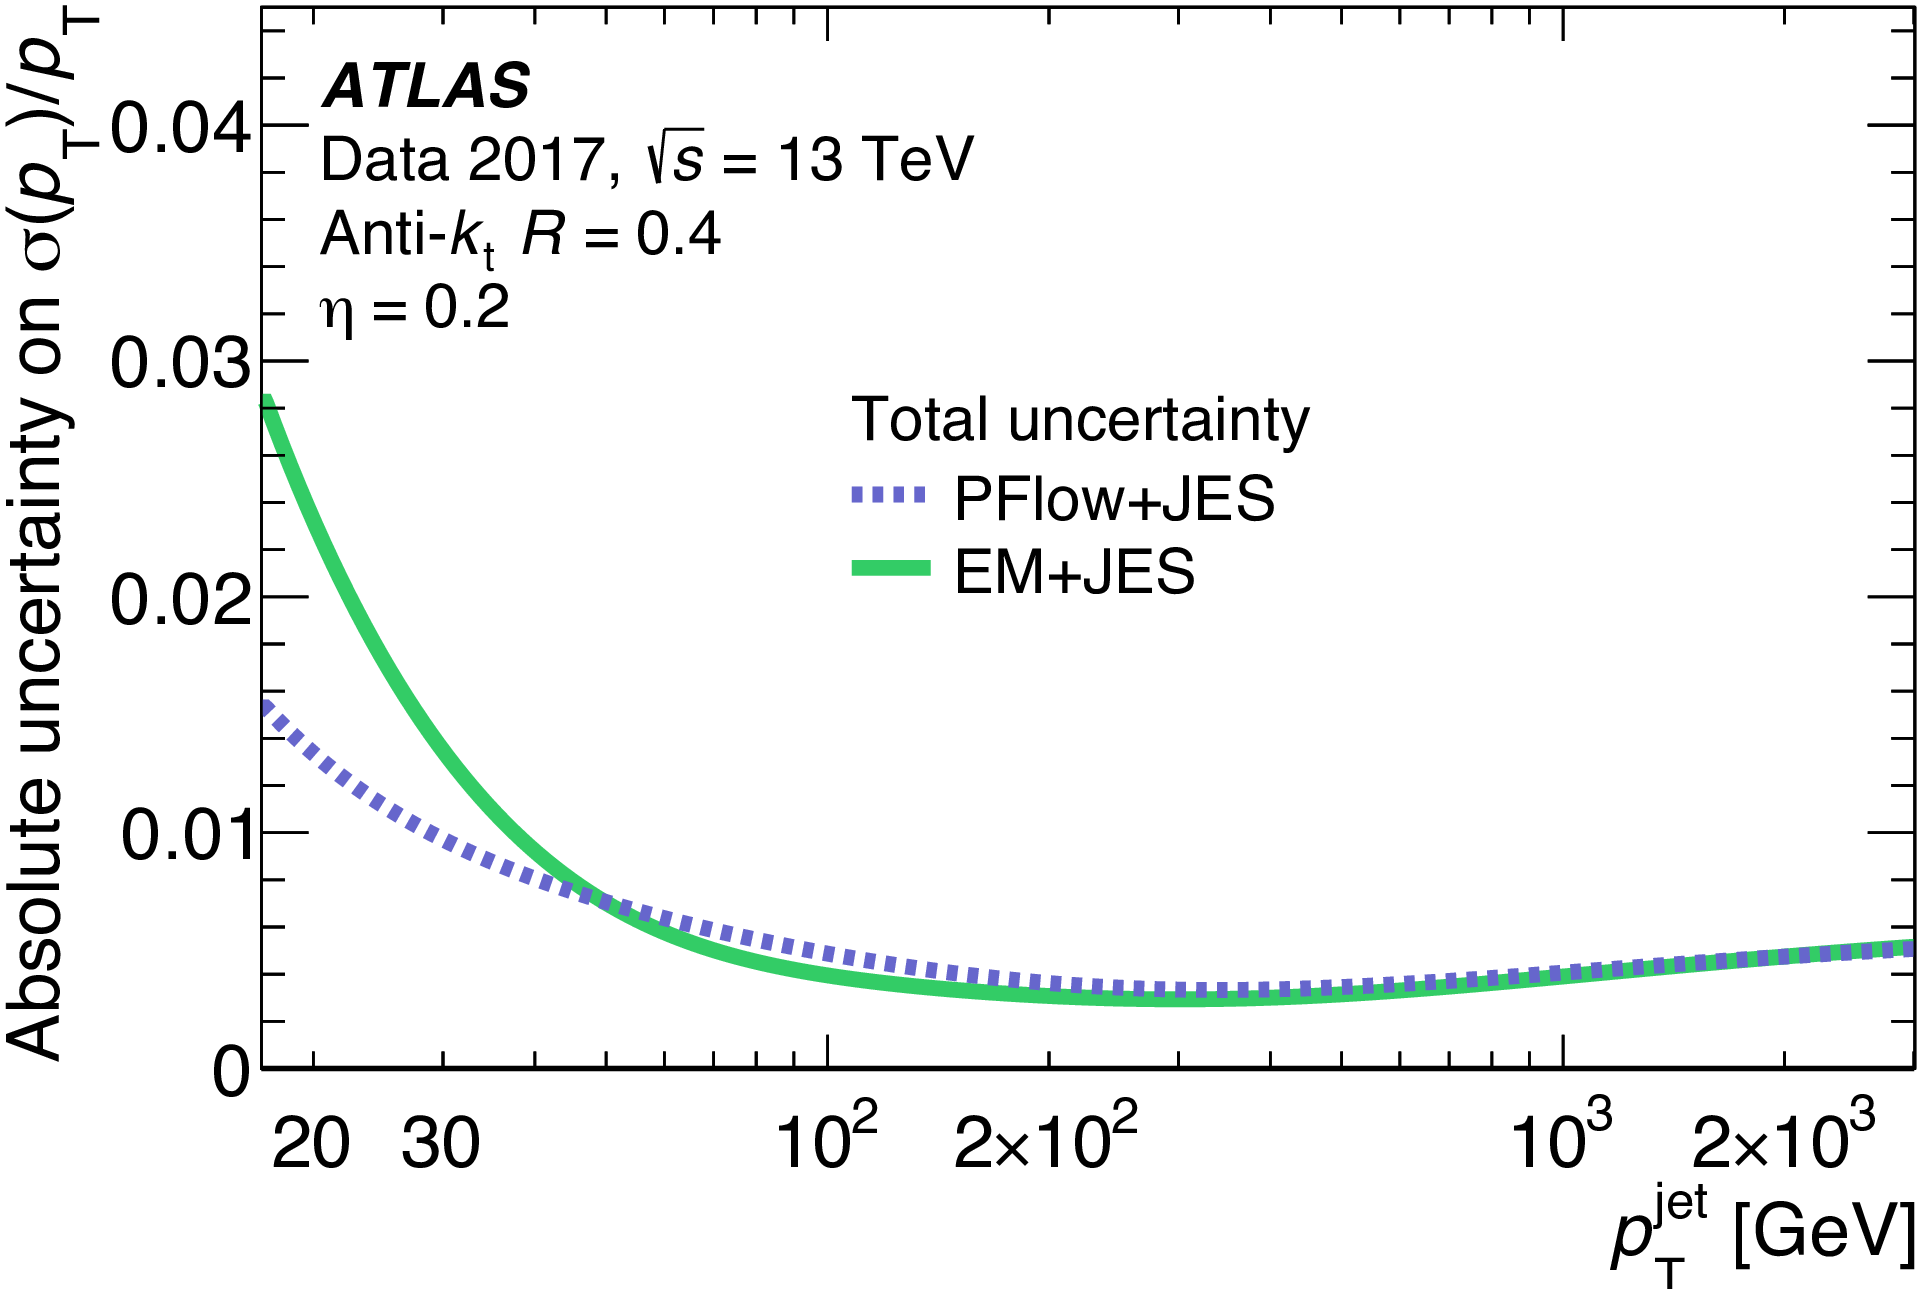
\includegraphics[width=\textwidth]{plots/atlas/JERa.png}
%    \caption{}
%    \label{fig:jer:a}
%\end{subfigure}
%\hfill
%\begin{subfigure}[b]{0.46\textwidth}
%    \centering
%    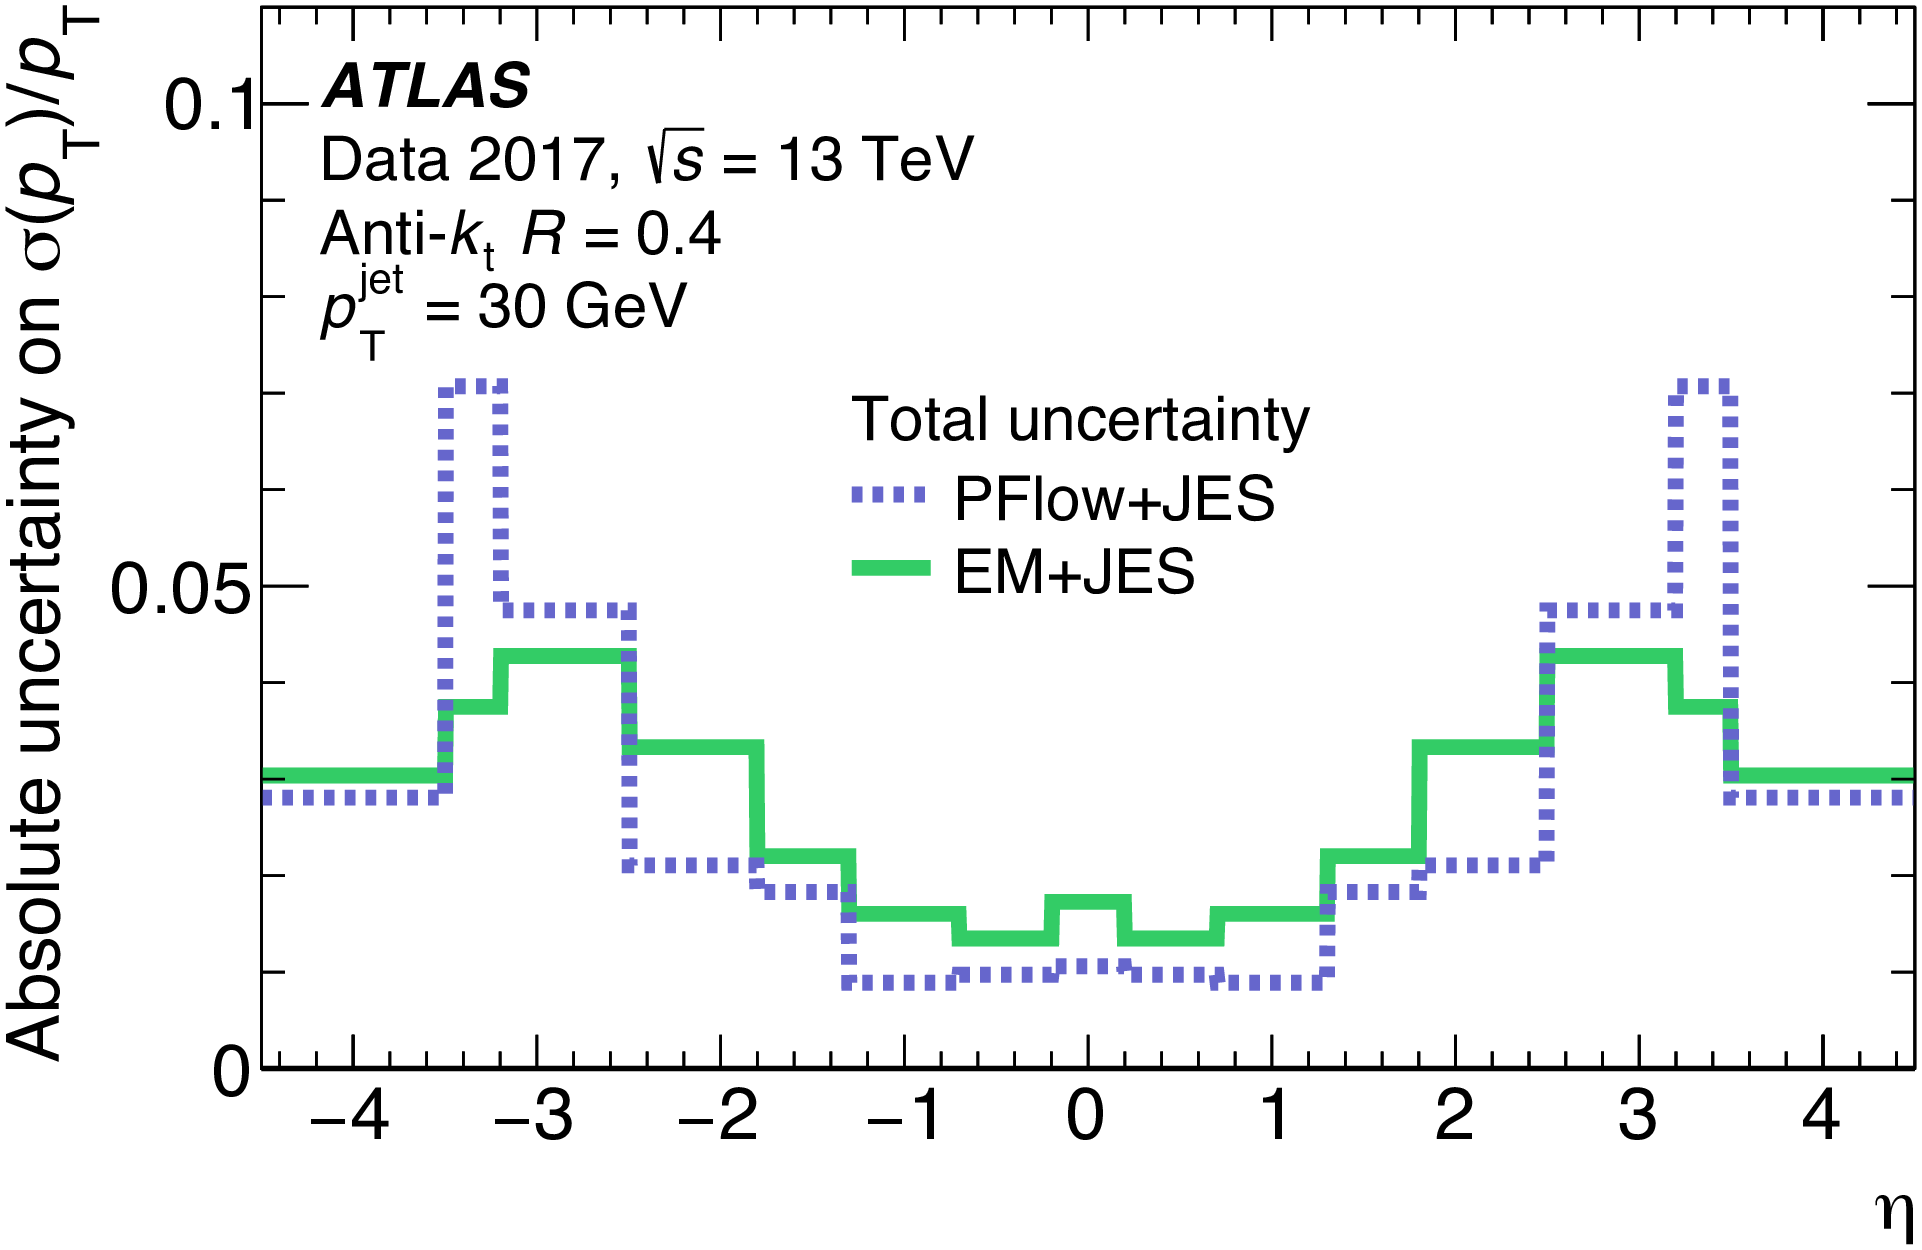
\includegraphics[width=\textwidth]{plots/atlas/JERb.png}
%    \caption{}
%    \label{fig:jer:b}
%\end{subfigure}
%\caption{Absolute uncertainty on the fractional JER for calibrated small-R PFlow and EMTopo jets for 2017 data. (a) shows the $\eta=0.2$ region with \pt. (b) shows the JER for 30\GeV jets with $\eta$. Figures from \cite{Atlas:smallrcali}.\label{fig:jer}}
%\end{figure}
%
\subsubsection{Jet Flavour Tagging}
Identifying jets containing $b$- and $c$-hadrons is very important in the context of precision electroweak measurements (for example \cite{Atlas:Hbb,Atlas:Hcc}). In the VBS measurement discussed in Chapter \ref{sec:vbswy}, $b$-tagging is of importance due to large backgrounds from top quarks, which decay to a $W$-boson and a $b$-quark. 

Because third generation quarks have a large CKM Suppression (little mixing between quark families), $b$-hadrons tend to have a large decay length. Furthermore, $b$-hadrons formed from the fragmentation of $b$-quarks tend to carry a large fraction of the intial quark momentum. This means that $b$-hadrons are likely to have a large Lorentz boost. The combination of these effects results in prominent displaced vertices. This detector signature is exploited in $b$-jet tagging algorithms, such as the \textit{DL1r} multivariate algorithm used for the $W\gamma$ VBS measurement \cite{Atlas:btagging}. When implementing $b$-tagging in an analysis, a tagging efficiency (the rate at which a true $b$-jet is identified correctly) working point needs to be selected depending on efficiency and purity requirements \cite{Buckley:PCP}. 

\subsubsection{Missing Tranverse Energy}

Since protons travelling along the LHC beamline carry no momentum component in the transverse plane, the \pt in any collision must be conserved. However, in many processes, an imbalance in momentum is expected due to the production of neutrinos which don't interact with the ATLAS detector, but can carry significant \pt. The missing transverse momentum \ptmiss is given by $\ptmiss\equiv(p^{\text{miss}}_x,p^{\text{miss}}_y)$ and quantifies the momentum balance in the transverse plane. The magnitude of the vector \ptmiss is referred to as the \textit{missing transverse energy} (MET), \met:
\begin{equation}\label{eq:etmiss_sum}
    \met = \sqrt{(p^{\text{miss}}_{\mathrm{x}})^2+(p^{\text{miss}}_{\mathrm{y}})^2}.
\end{equation}
The direction of the \ptmiss in the transverse plane is defined as
\begin{equation}
    \phi^{\text{miss}}=\text{atan2}(p_y^{\text{miss}},p_x^{\text{miss}}),
\end{equation}
where the atan2$(y,x)$ function is defined to return the argument of the complex number $x+iy$, and is used over the arctan function as it covers the interval $(-\pi,\pi]$, rather than the $[-\frac{\pi}{2},\frac{\pi}{2}]$ interval covered by the arctan function.

The components $p^{\text{miss}}_{x(y)}$ are given by the negative vector sum of \textit{hard objects} and \textit{soft signals} in the event:
\begin{equation}
    p^{\text{miss}}_{x(y)}=-\sum_{i\in\{\text{hard objects}\}}p_{x(y),i}-\sum_{j\in\{\text{soft signals}\}}p_{x(y),j}.
\end{equation} 
The \textit{hard objects} refer to electrons, photons, muons, $\tau$ leptons, and jets, with a set of kinematic and object reconstruction quality requirements. The \textit{soft signals} refers to all detector signals for the triggered event which do not contribute to the hard objects. They include non-collision backgrounds such as scattered soft particles from the UE as well as signals from objects which do not satisfy the hard object selection criteria. 

The mutual exclusivity of the detector signal requires a well defined sequence of contributions as well a way of rejecting signals where overlaps are present. The usual reconstruction sequence for the hard objects is electron reconstruction, followed by photons, hadronically decaying $\tau$s, muons, and finally jets. Each of these objects are fully calibrated before they enter the \ptmiss calclation, such that contributions to \ptmiss do not arise due to incorrect energy scales. All electrons passing some selection criteria are included in the \ptmiss reconstruction first, and particles further in the sequence are rejected if there is a shared calorimeter signal with an earlier particle in the sequence. 

The contributions from soft signal are calculated in the following way. Good quality tracks in \pt range of $400\MeV<\pt<100\GeV$ are selected. The tracks are then extrapolated to a high granularity region of the EM calorimeter, and a $\Delta R$ check is performed to assess whether the track is associated with an calorimeter deposits. Those tracks which do not have calorimeter deposits are retained in the soft term, and those which do match to a topo-cluster, are also retained, but the topo-cluster is removed in order to take advantage of the improved \pt resolution of the ID. For cases where multiple topo-clusters are matched to a given track, the highest energy cluster is retained. Any left over topo-clusters which have not been matched to tracks or discarded are also added to the soft term. The performance of \met and \ptmiss reconstruction is assessed using $Z\rightarrow ee/\mu\mu$ events, where selections of the dilepton invariant mass around the $Z$ invariant mass peak provide clean signal with no expected contributions for \met. Events involving leptonic $W$ decays in association with jets are used to study cases with true \MET \cite{Buckley:PCP,Atlas:met}. % The signals from muons are unique in that, in most cases, they are reconstructed solely from ID and MS contributions, as such the decision of where muons are reconstructed in this sequence is of little importance.
%The Missing Transverse Energy (MET), \met, is defined using the components $E_{\mathrm{x(y)}}^{\text{miss}}$ along the $x$ and $y$ axes: 
%\begin{equation}\label{eq:etmiss_xy}
%  E_{\mathrm{x(y)}}^{\text{miss}}=E_{\mathrm{x(y)}}^{\text{miss},e}+E_{\mathrm{x(y)}}^{\text{miss},\mu}+E_{\mathrm{x(y)}}^{\text{miss},\gamma}+E_{\mathrm{x(y)}}^{\text{miss,jets}}+E_{\mathrm{x(y)}}^{\text{miss,Soft-Term}},
%\end{equation}
%where each term is defined as the magnitude of the negative vector sum of the reconstructed objects passing the preselection cuts, projected on to the $x$ or $y$ axis. The "Soft-Term" component is calculated entirely from primary vertex tracks not matched to the physics objects associated with the other "Hard-Terms". This is the "Track Soft-Term", or TST. Since tracks can be matched to a primary vertex, the TST \met is relatively robust to pile-up contributions.

%The \met is calculated using calibrated physics objects, meaning corrections applied to the physics objects are taken into account in the \met calculation. The preselection cuts on the physics objects defining the hard terms are: $\pt^{\gamma}>12\GeV$, $\pt^{e(\mu)}>7\GeV$, and $\pt^{\text{jet}}>25\GeV$. The Tight working point is used in which forward jets are required to have $pT > 30$.%The baseline fiducial region has a cut on the MET of $\met > 30GeV$.

\subsubsection{Taus}
Tau leptons decay (decay length $87\mu\text{m}$) either leptonically or hadronically before reaching the active parts of the ATLAS detector. About 35\% of the time, taus decay to a tau neutrino, electron/muon, and lepton neutrino mediated via an off-shell $W$ boson. 65\% of the decay modes involve the tau decaying hadronically, where in 72\% and 22\% of the time one or three charged pions are produced, respectively. Additionally, 68\% of hadronic tau decays involve the production of a neutral pion. Leptonic tau decays cannot be distinguished from electrons or muons at the interaction point, however hadonic tau decays have a very specific signature. Firstly, the invariant mass of the system of jets must be less than the tau invariant mass of around 1.8\GeV, and the predictable production of charged pions result in either one or three tracks in the ID \cite{Atlas:trackmultiplicity}. Taus also have very collimated showers compared to QCD jets, this is because QCD jets are initiated by partons carrying colour charge, where the hadronisation process results in multiple quark and gluon emissions due to them being colour-connected to the initial parton. Additionally, tau tracks tend to have large impact parameters due to the significant decay length of the tau. Taus are reconstructed initially as jets using the anti-$k_t$ with $R=0.4$. Afterwards, a multivariate analysis uses various jet properties to tag the taus \cite{Buckley:PCP,Atlas:tau}. 
\begin{figure}[t]
   \centering
   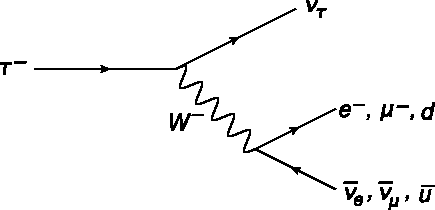
\includegraphics[width=0.5\textwidth]{plots/atlas/taudecay.pdf} 
   \caption{Feynman diagram for tau decays via off-shell $W$ boson. From \cite{Buckley:PCP}. \label{fig:taudecay}}
\end{figure}